\subsection{การทดลองการเดิน}
การทดลองการเดินนั้นได้ทดลองด้วยการปรับค่าข้อต่อให้เหมาะสมแก่การเดิน เพื่อทดสอบโครงสร้างที่ได้ออกแบบ
มาว่าสามารถรองรับการเดินของหุ่นยนต์ได้จริงหรือไม่ โดยค่าที่ใช้ในการปรับนั้นจะเป็นค่ามุมของมอเตอร์ส่วนต่างๆของส่วนขาทั้ง 2 ข้าง
โดยจะตั้งชื่อมอเตอร์ตามแกนของข้อต่อแต่ละส่วนโดยเริ่มจากส่วนจะโพกจะมี 3 แกนคือ hip yaw,hip roll,hip pitch ส่วนหัวเข่า 1 แกนคือ
knee pitch และส่วนข้อเท้า 2 แกนคือ ankle pitch,ankle roll โดยในขาแต่ละข้างจะแยกด้วยสัญลักษณ์ Right(ขาข้างขวา)และ Left(ขาข้างซ้าย)
โดยอิงจากตัวของหุ่นยนต์ และสั่งงานให้ไปตามมุมต่างๆที่กำหนดไว้ดังภาพ 

\subsubsection*{รูปกราฟแสดงตำแหน่งมอเตอร์ขาขวา}
\begin{figure}[!ht]
  \centering
  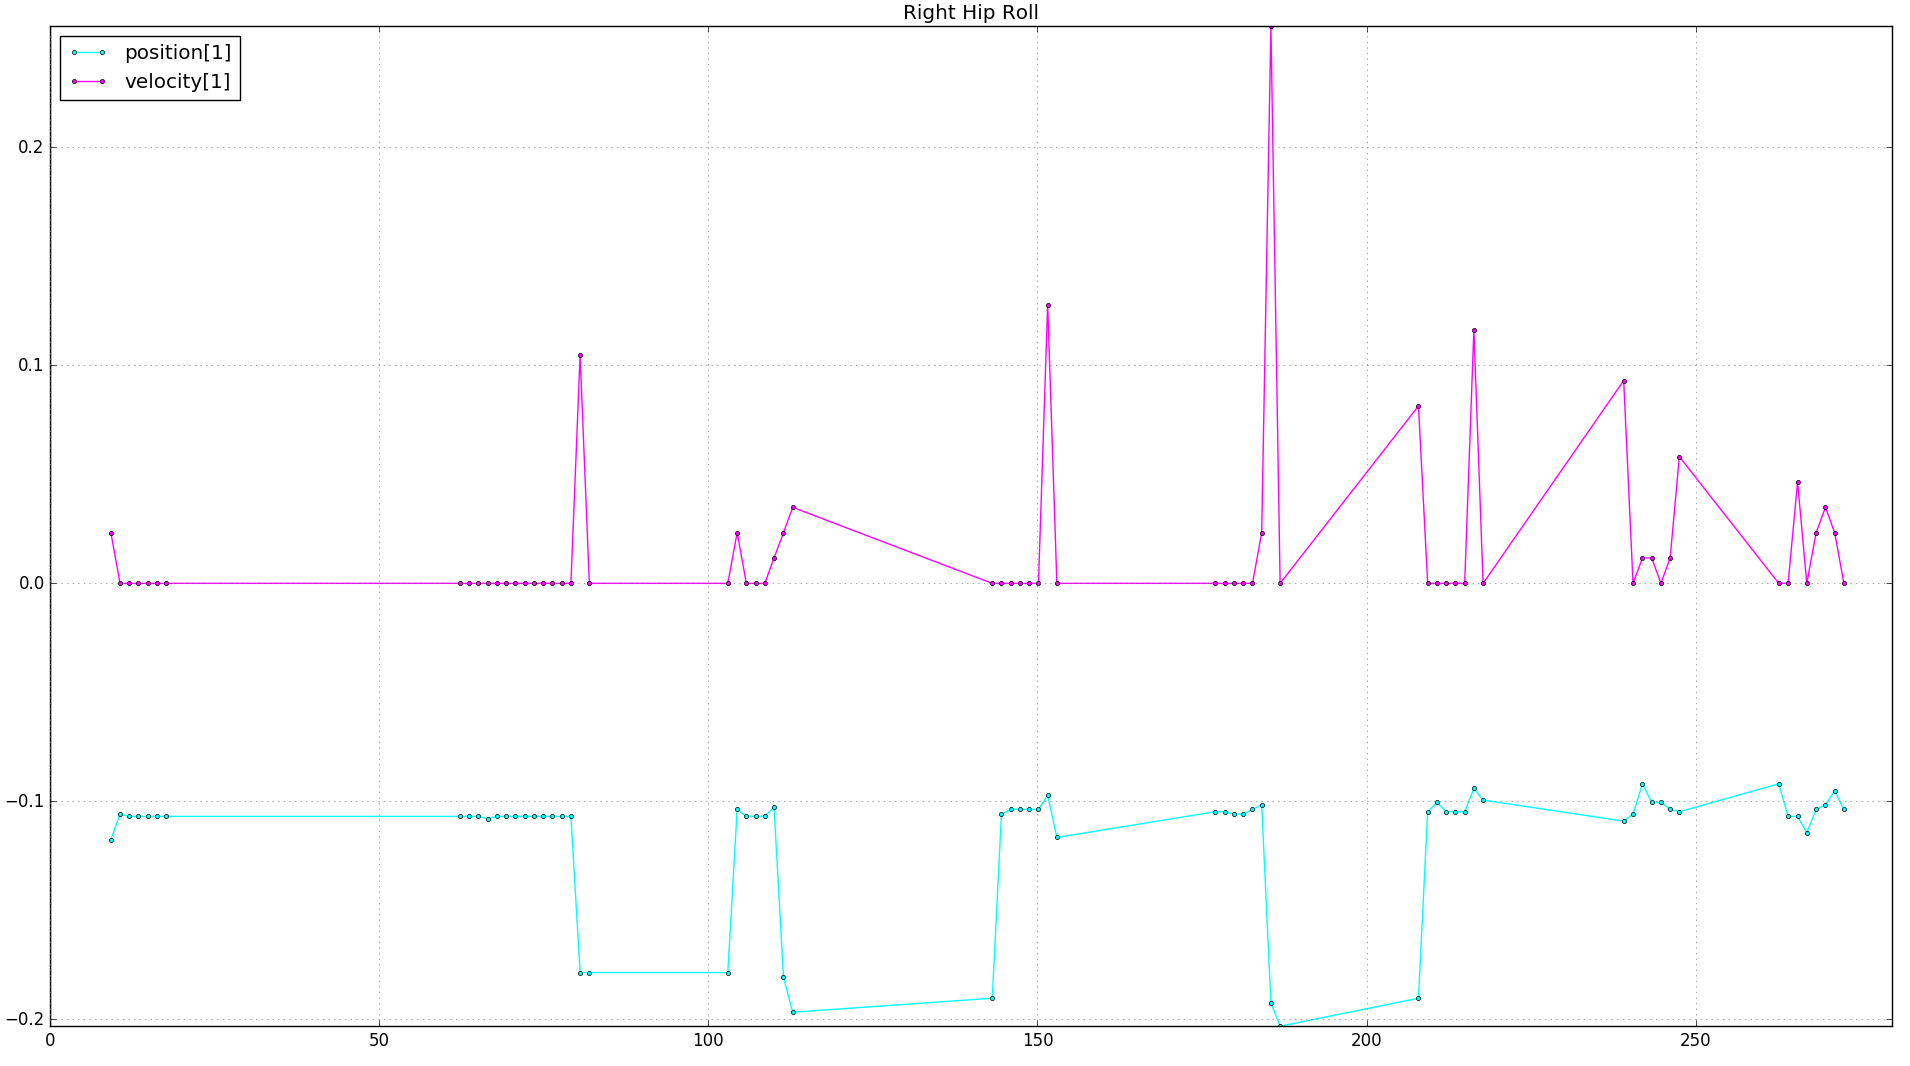
\includegraphics[width=1.0\linewidth]{chapter4/images/right_hip_roll.png}
  \caption{รูปการสั่งงานข้อต่อ right hip roll}
  \label{fig:right_hip_roll}
\end{figure}
\clearpage

\begin{figure}[!ht]
  \centering
  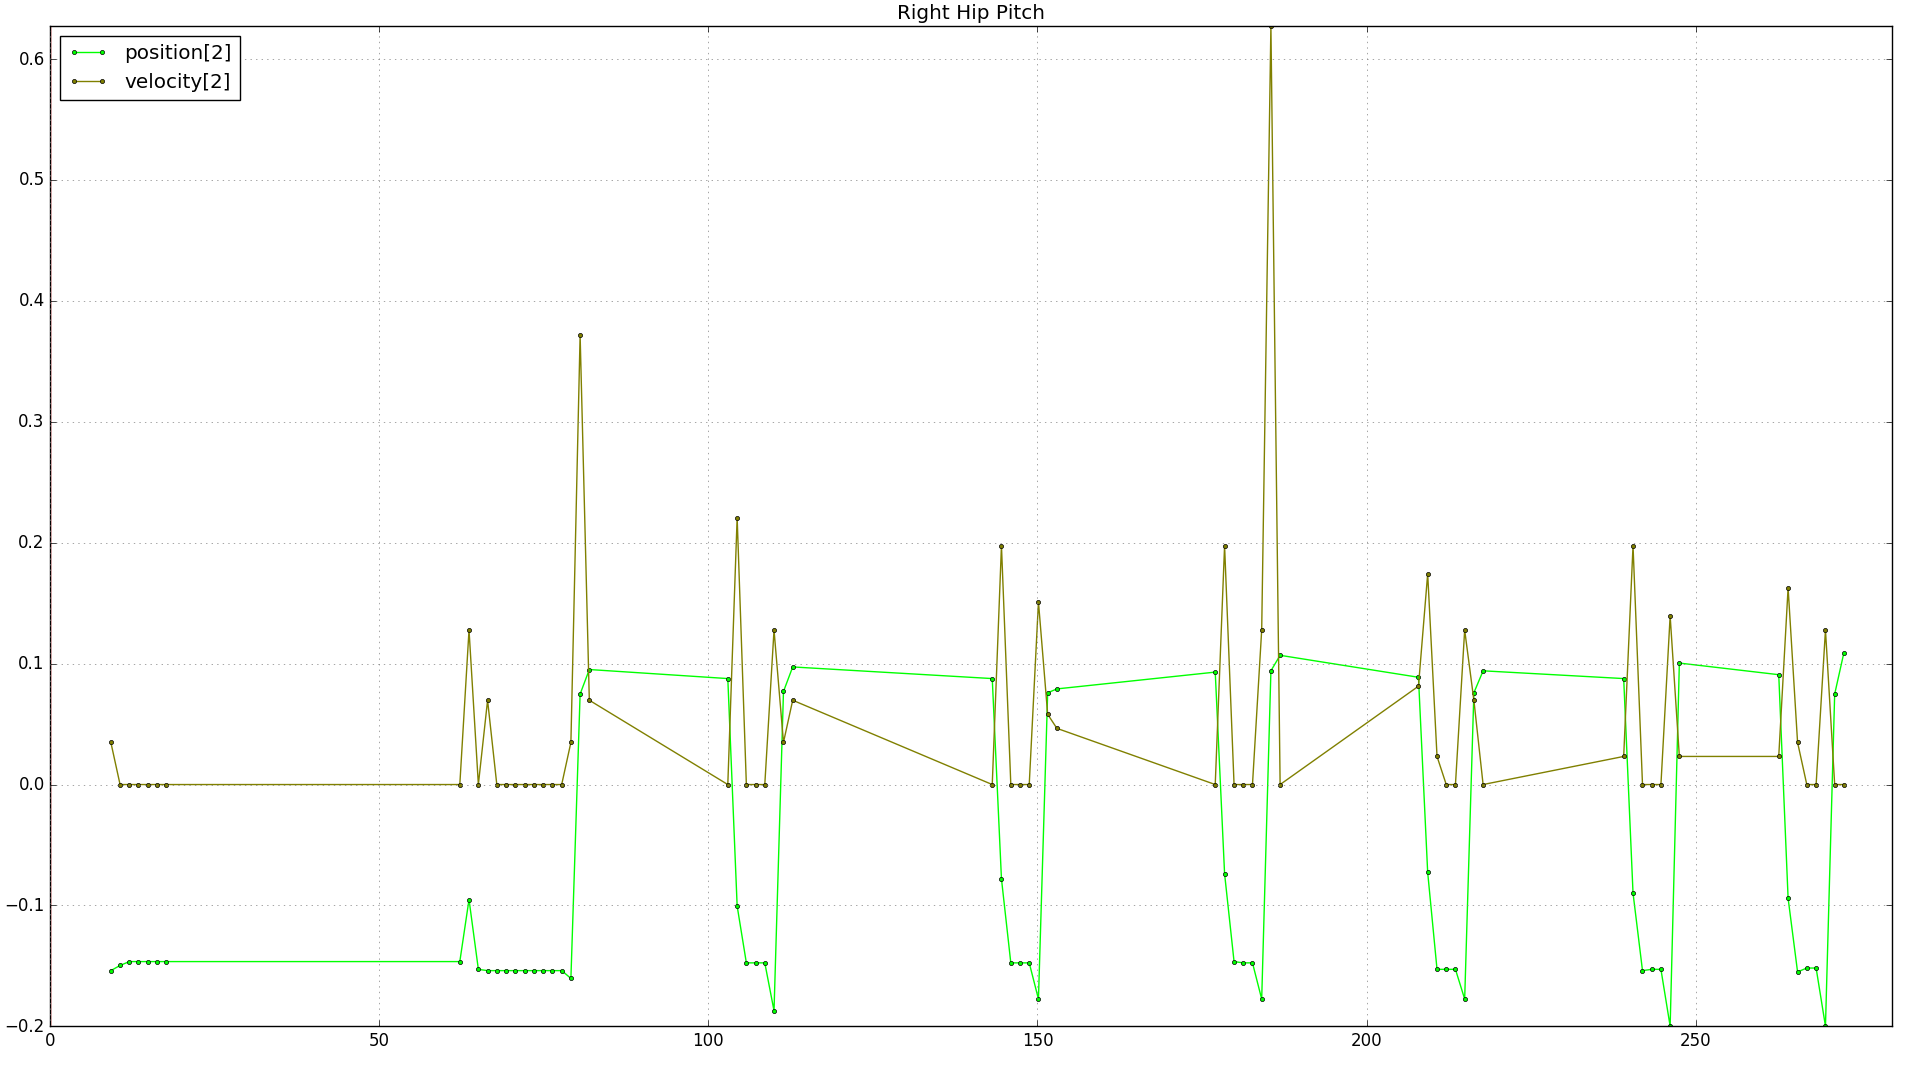
\includegraphics[width=1.0\linewidth]{chapter4/images/right_hip_pitch.png}
  \caption{รูปการสั่งงานข้อต่อ right hip pitch}
  \label{fig:right_hip_pitch}
\end{figure}

\begin{figure}[!ht]
  \centering
  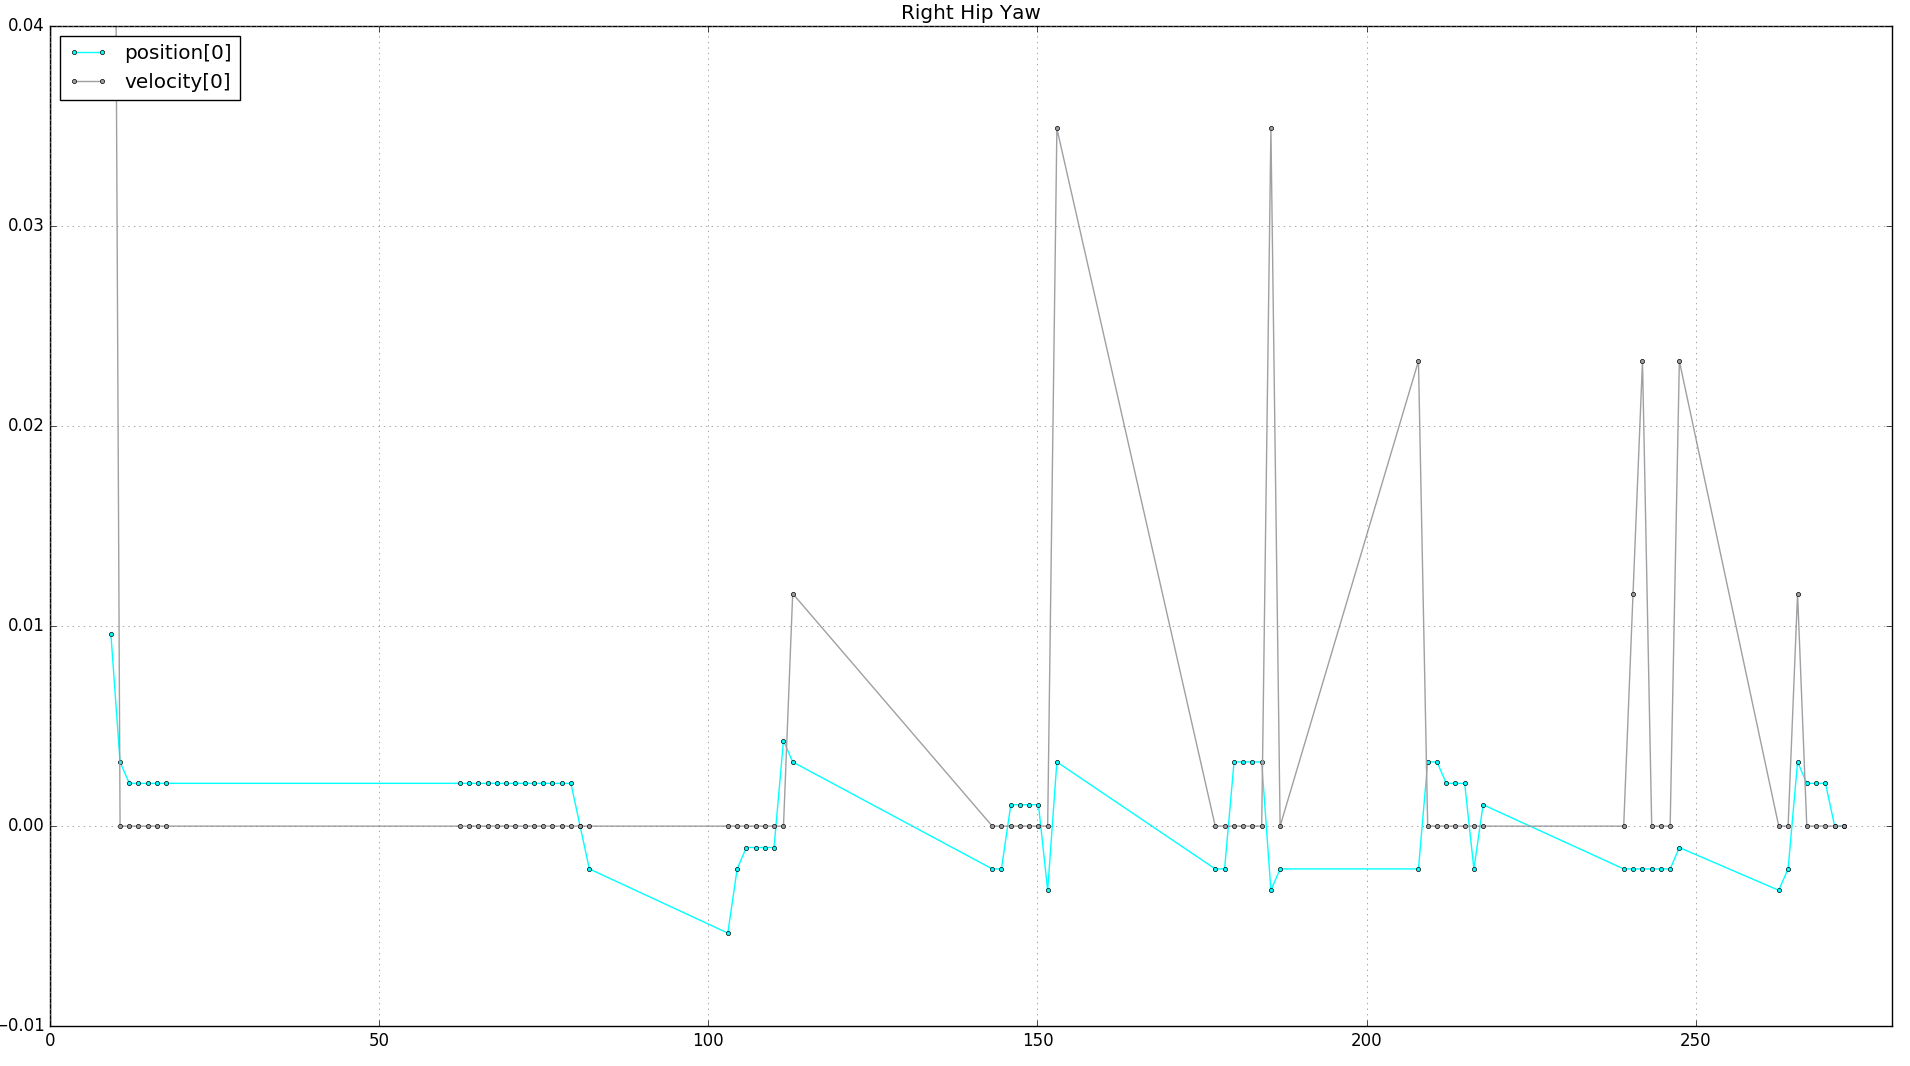
\includegraphics[width=1.0\linewidth]{chapter4/images/right_hip_yaw.png}
  \caption{รูปการสั่งงานข้อต่อ right hip yaw}
  \label{fig:right_hip_yaw}
\end{figure}
\clearpage

\begin{figure}[!ht]
  \centering
  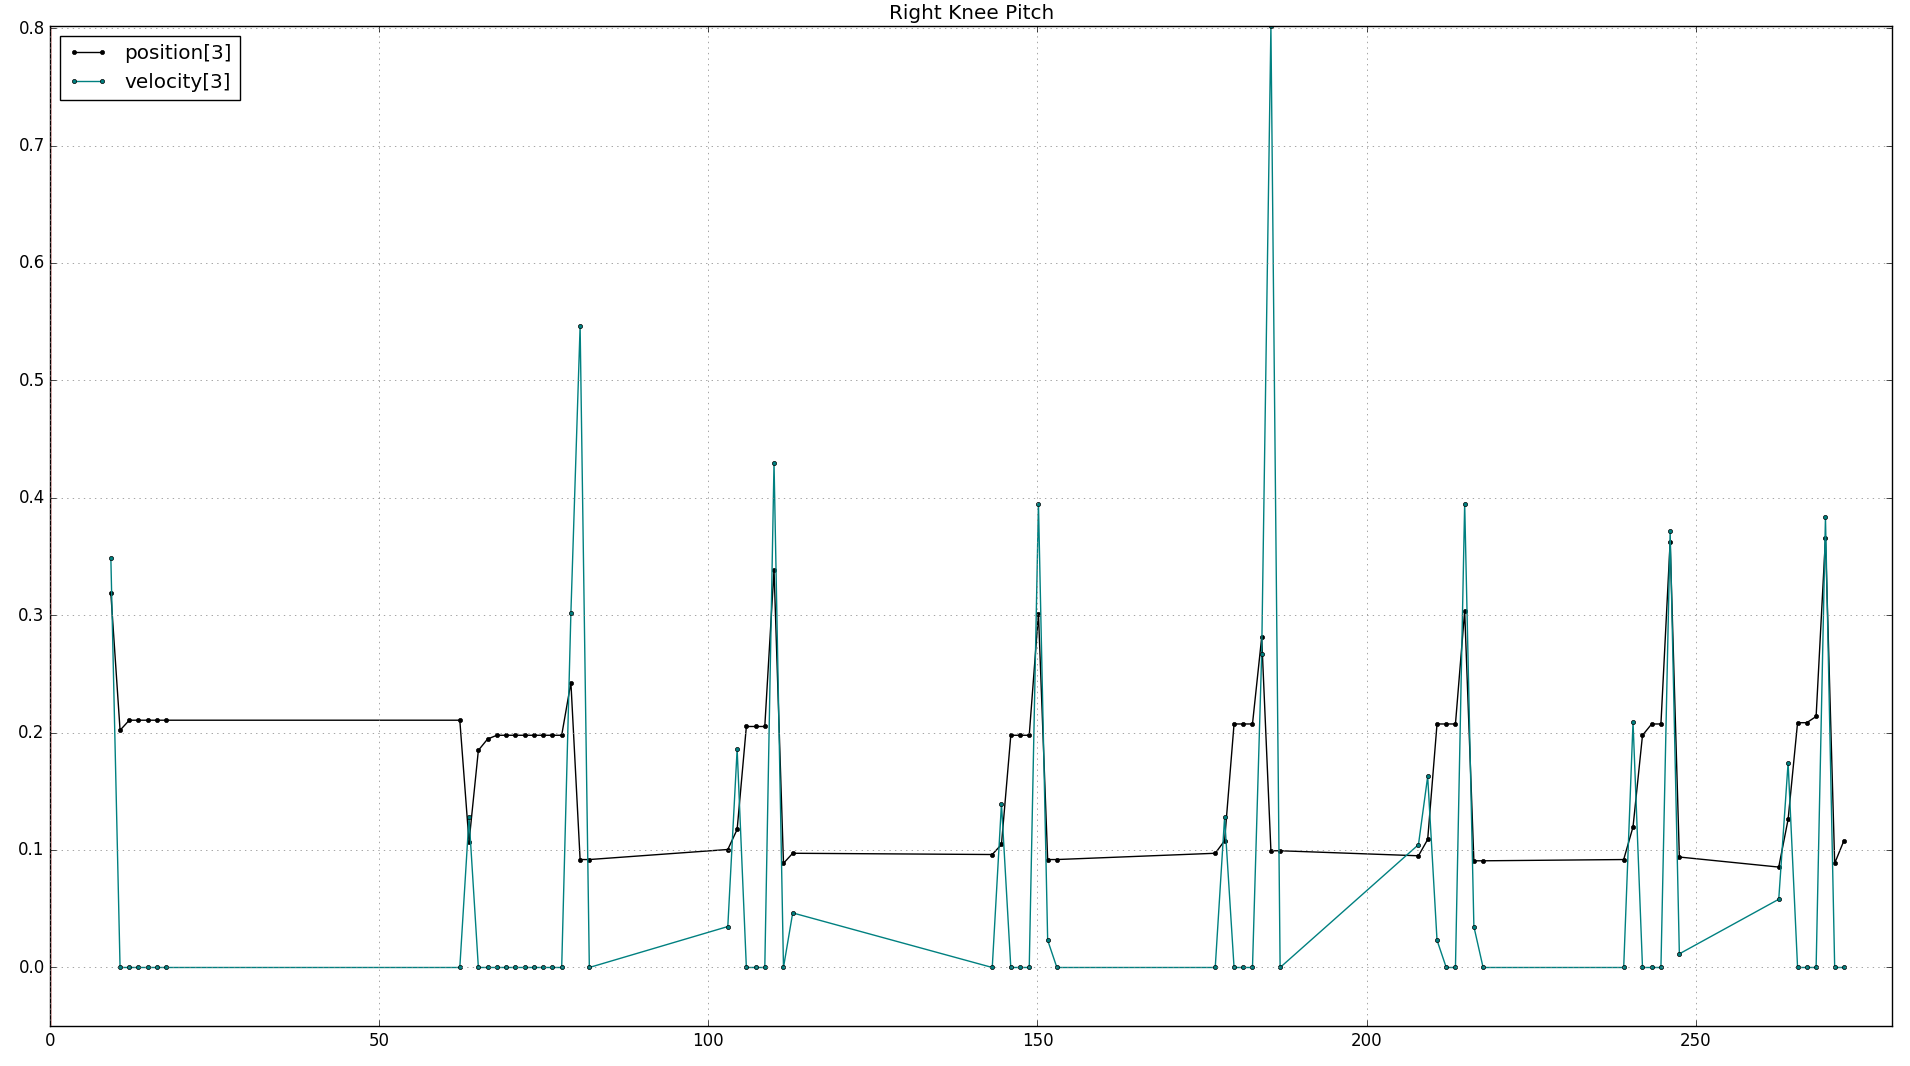
\includegraphics[width=1.0\linewidth]{chapter4/images/right_knee_pitch.png}
  \caption{รูปการสั่งงานข้อต่อ right knee pitch}
  \label{fig:right_knee_pitch}
\end{figure}

\begin{figure}[!ht]
  \centering
  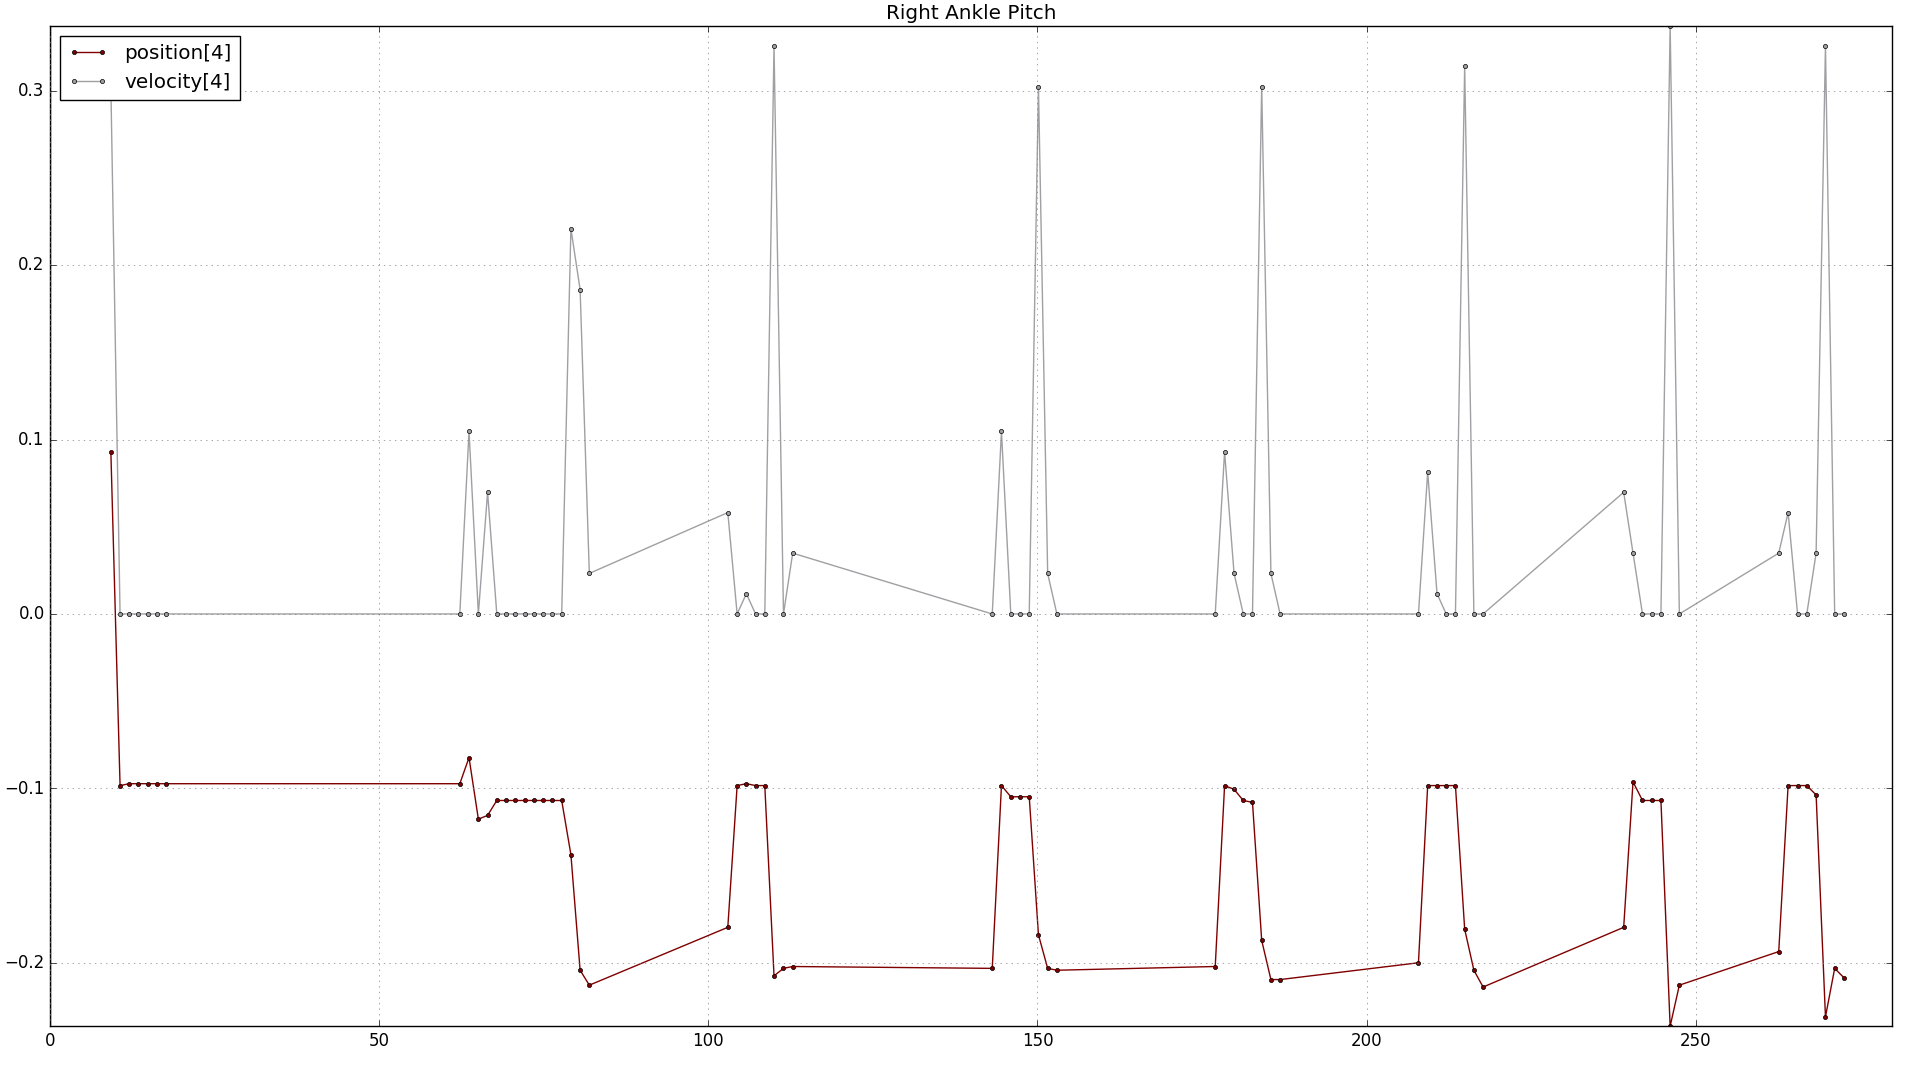
\includegraphics[width=1.0\linewidth]{chapter4/images/right_ankle_pitch.png}
  \caption{รูปการสั่งงานข้อต่อ right ankle pitch}
  \label{fig:right_ankle_pitch}
\end{figure}
\clearpage

\begin{figure}[!ht]
  \centering
  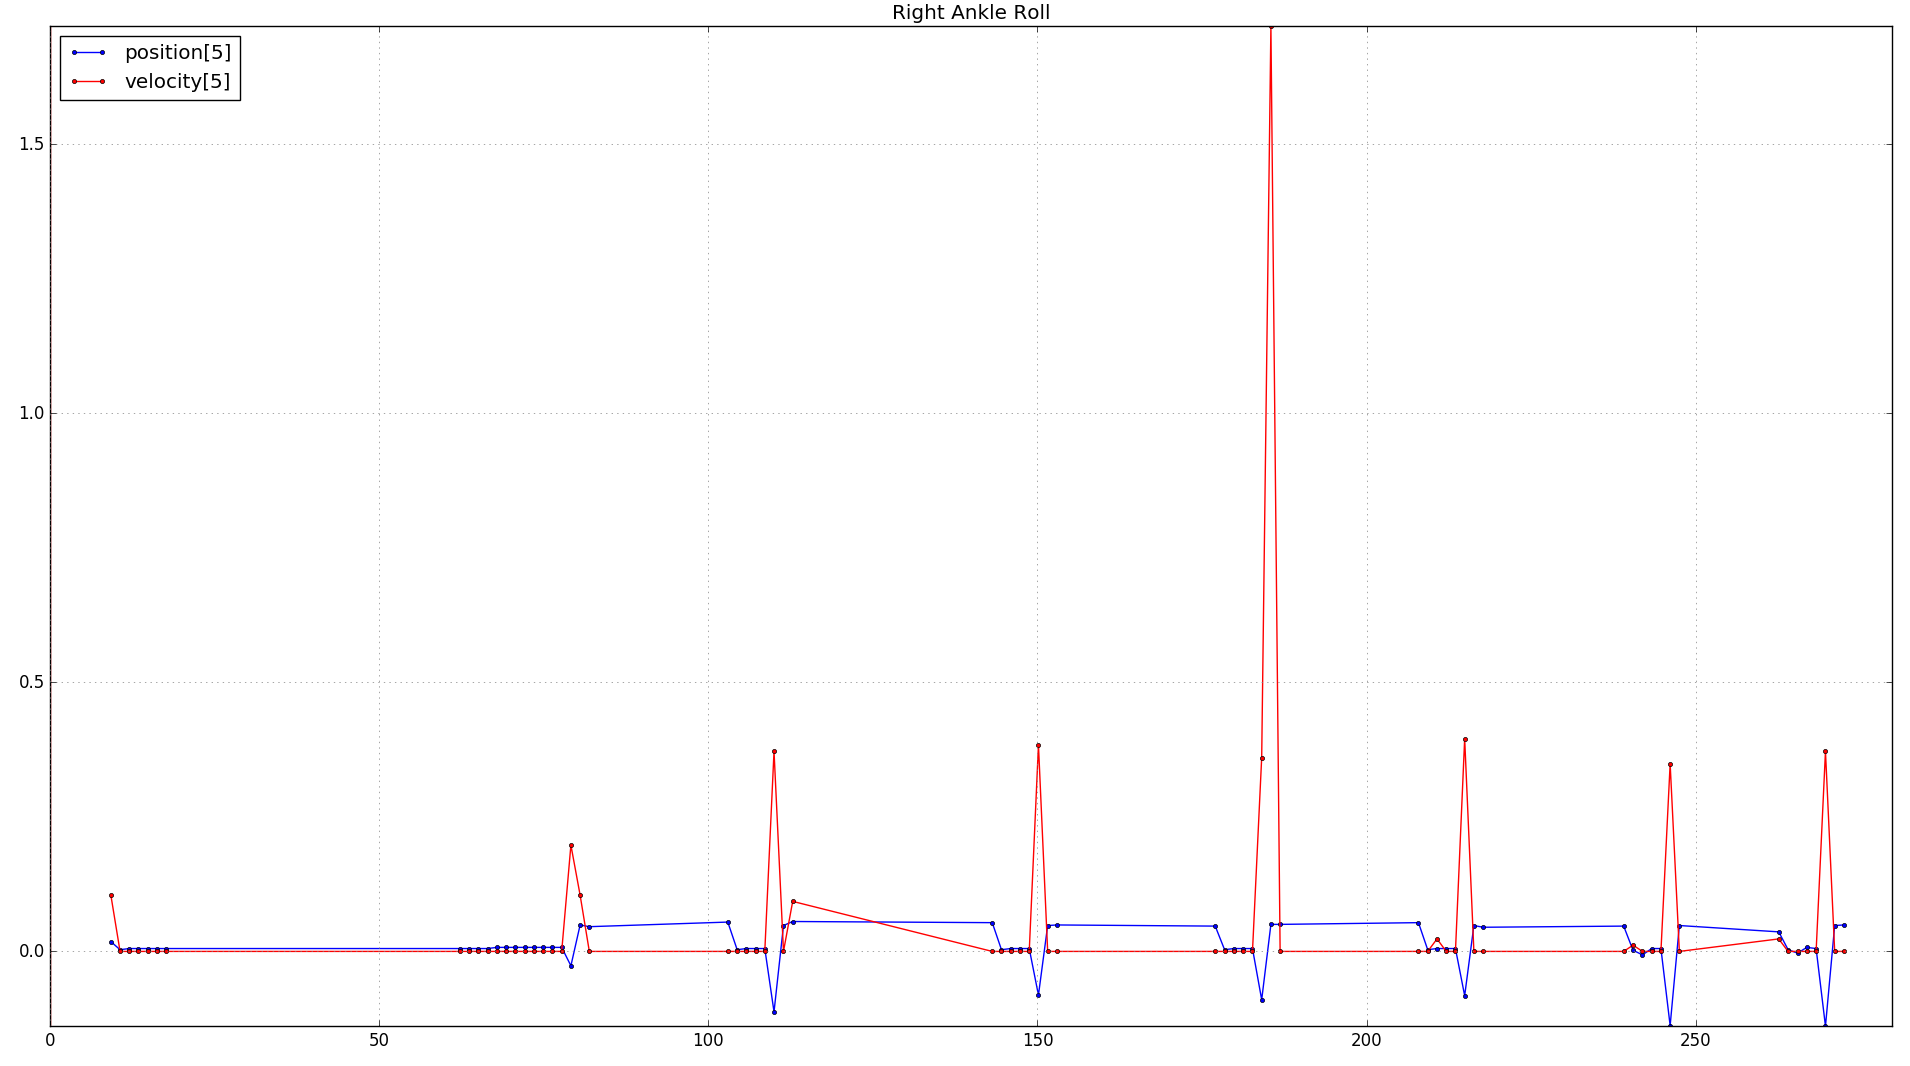
\includegraphics[width=1.0\linewidth]{chapter4/images/right_ankle_roll.png}
  \caption{รูปการสั่งงานข้อต่อ right ankle roll}
  \label{fig:right_ankle_roll}
\end{figure} 
\clearpage
  
\subsubsection*{รูปกราฟแสดงตำแหน่งมอเตอร์ขาซ้าย}
\begin{figure}[!ht]
  \centering
  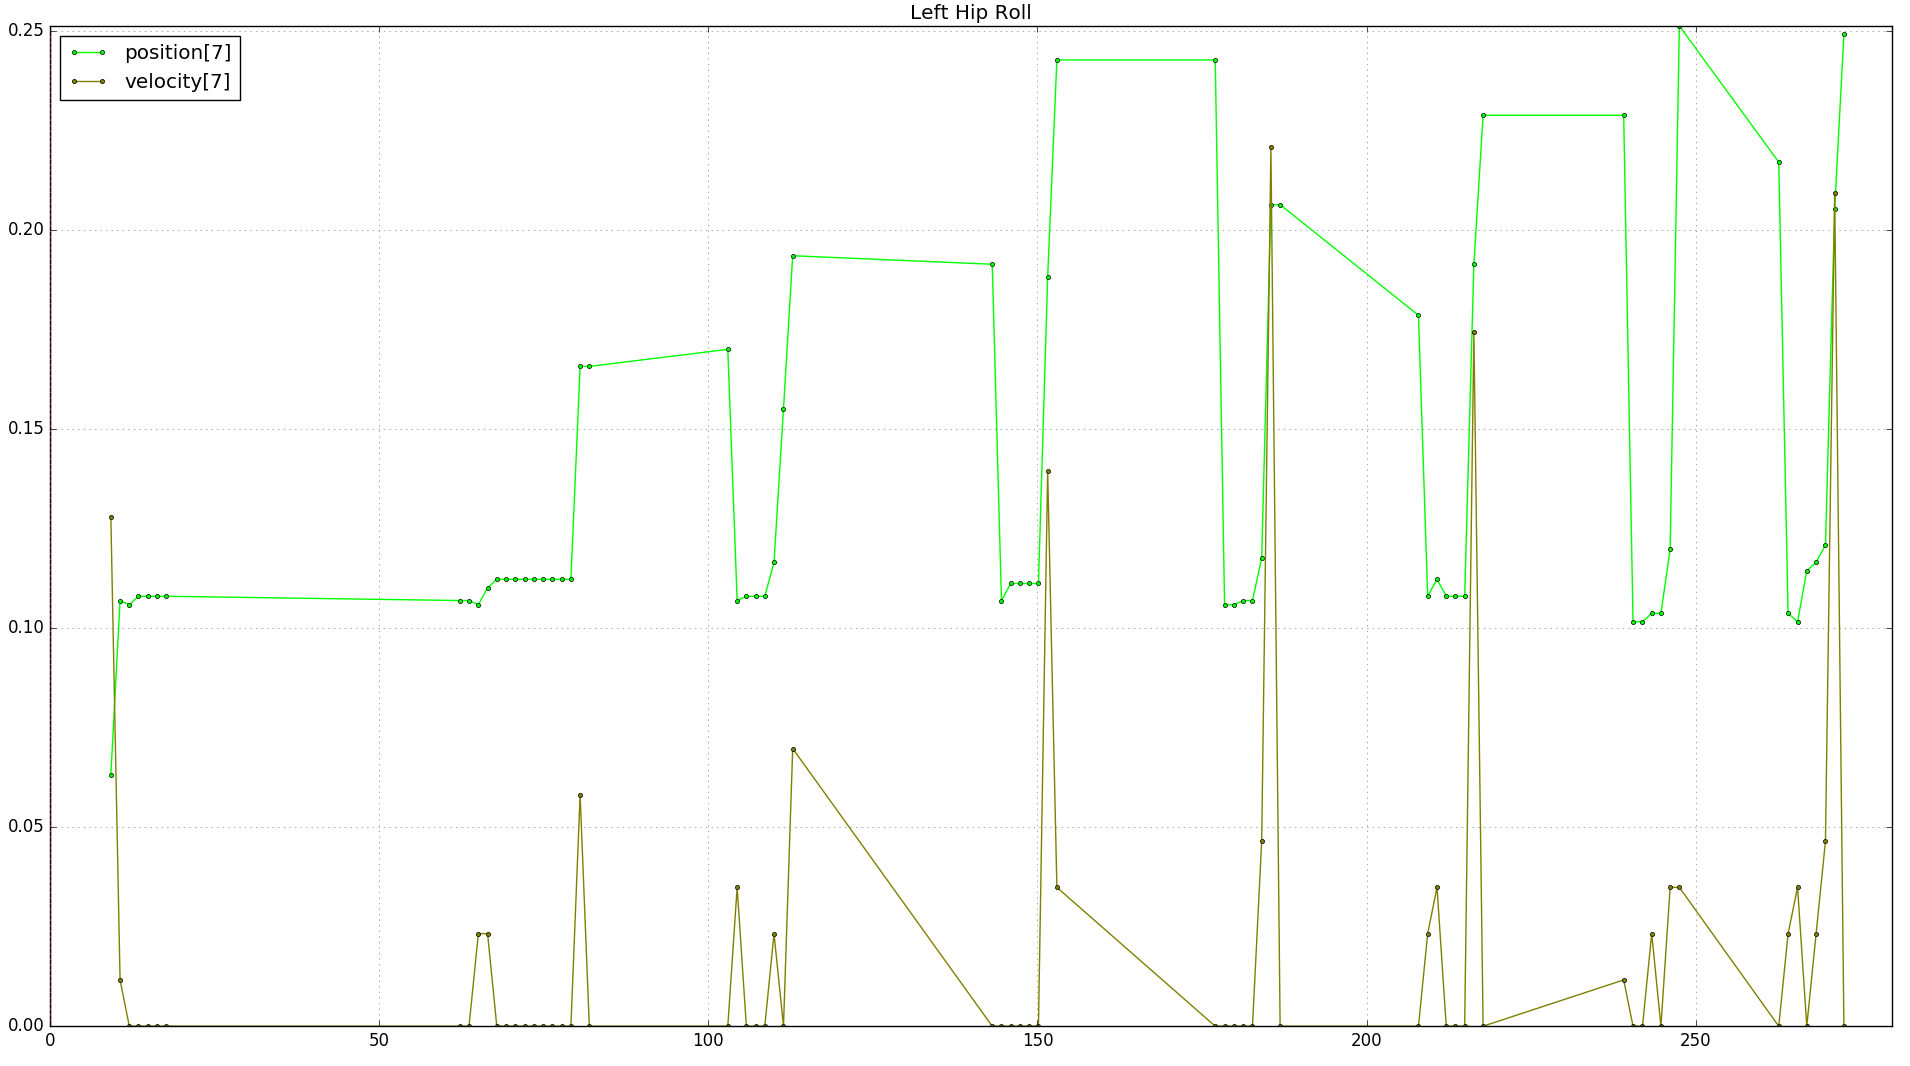
\includegraphics[width=1.0\linewidth]{chapter4/images/left_hip_roll.png}
  \caption{รูปการสั่งงานข้อต่อ left hip roll}
  \label{fig:left_hip_roll}
\end{figure}

\begin{figure}[!ht]
  \centering
  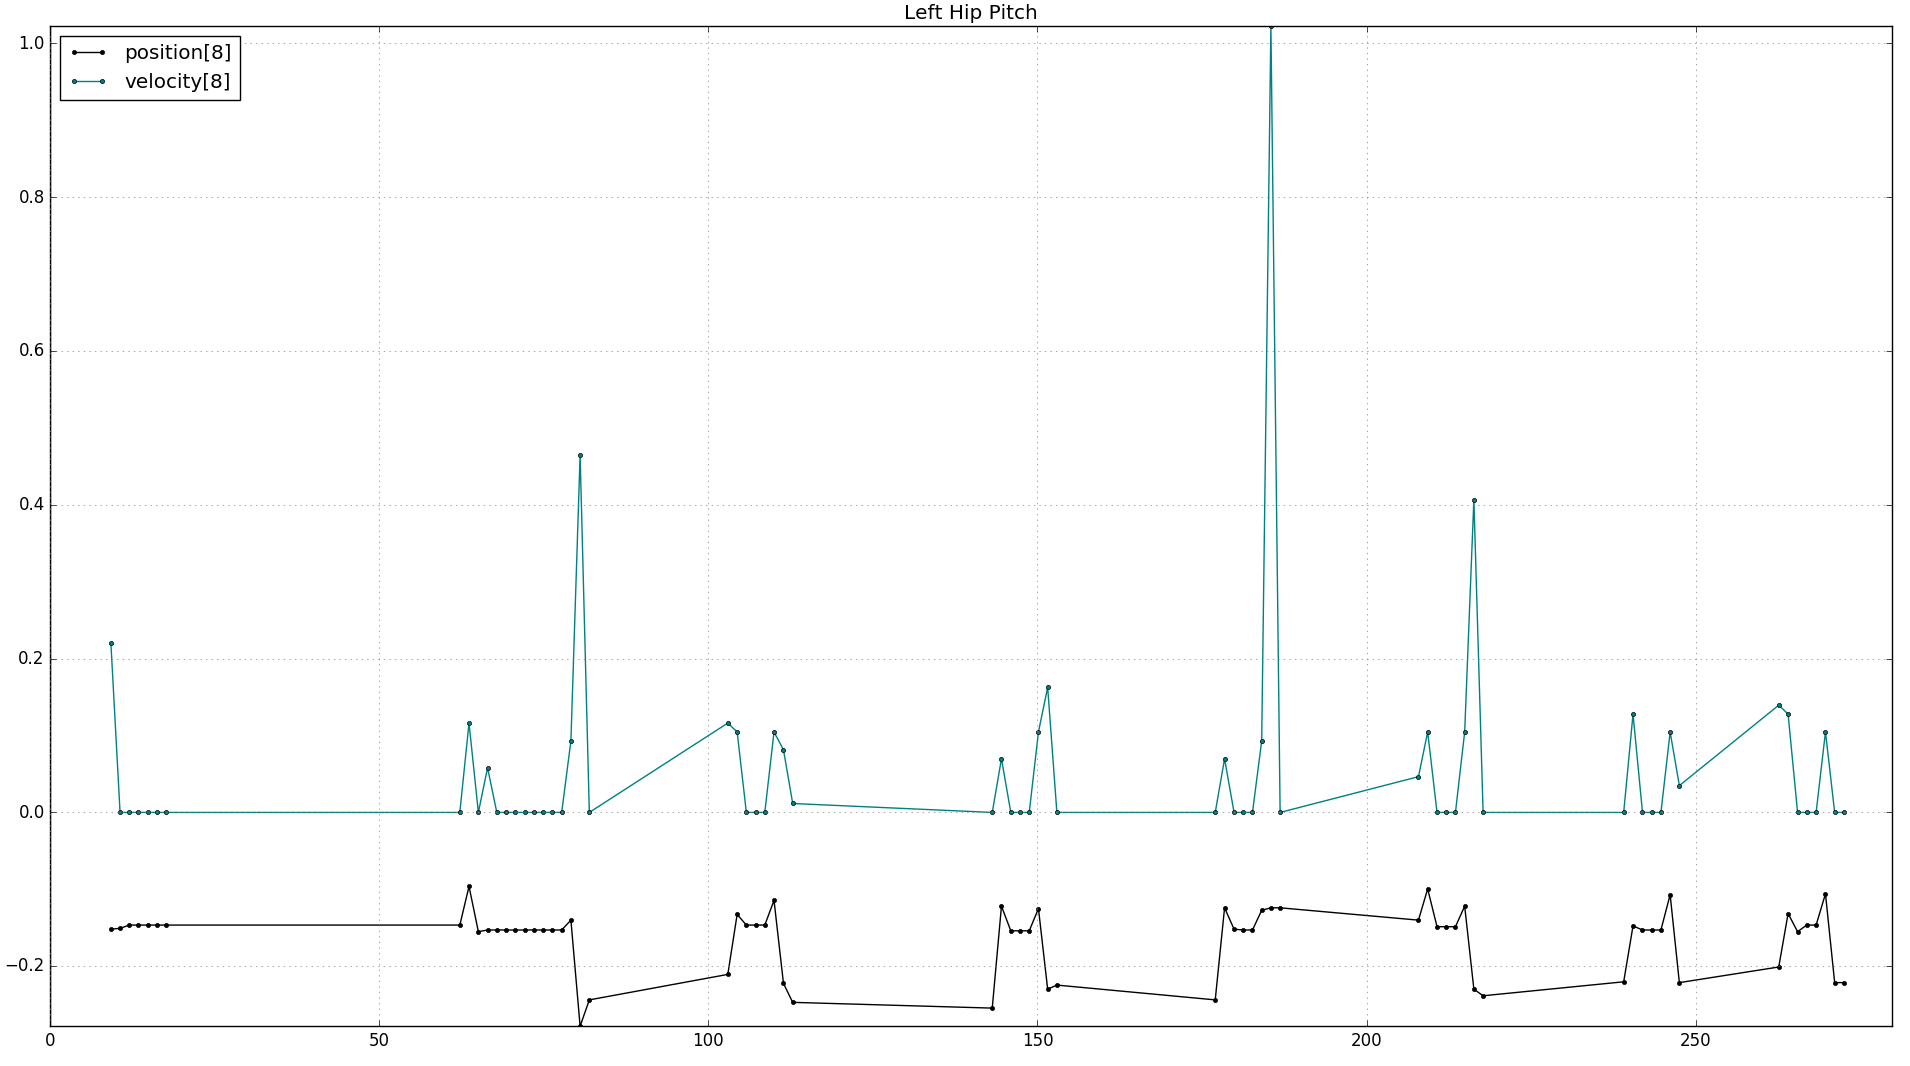
\includegraphics[width=1.0\linewidth]{chapter4/images/left_hip_pitch.png}
  \caption{รูปการสั่งงานข้อต่อ left hip pitch}
  \label{fig:left_hip_pitch}
\end{figure}
\clearpage

\begin{figure}[!ht]
  \centering
  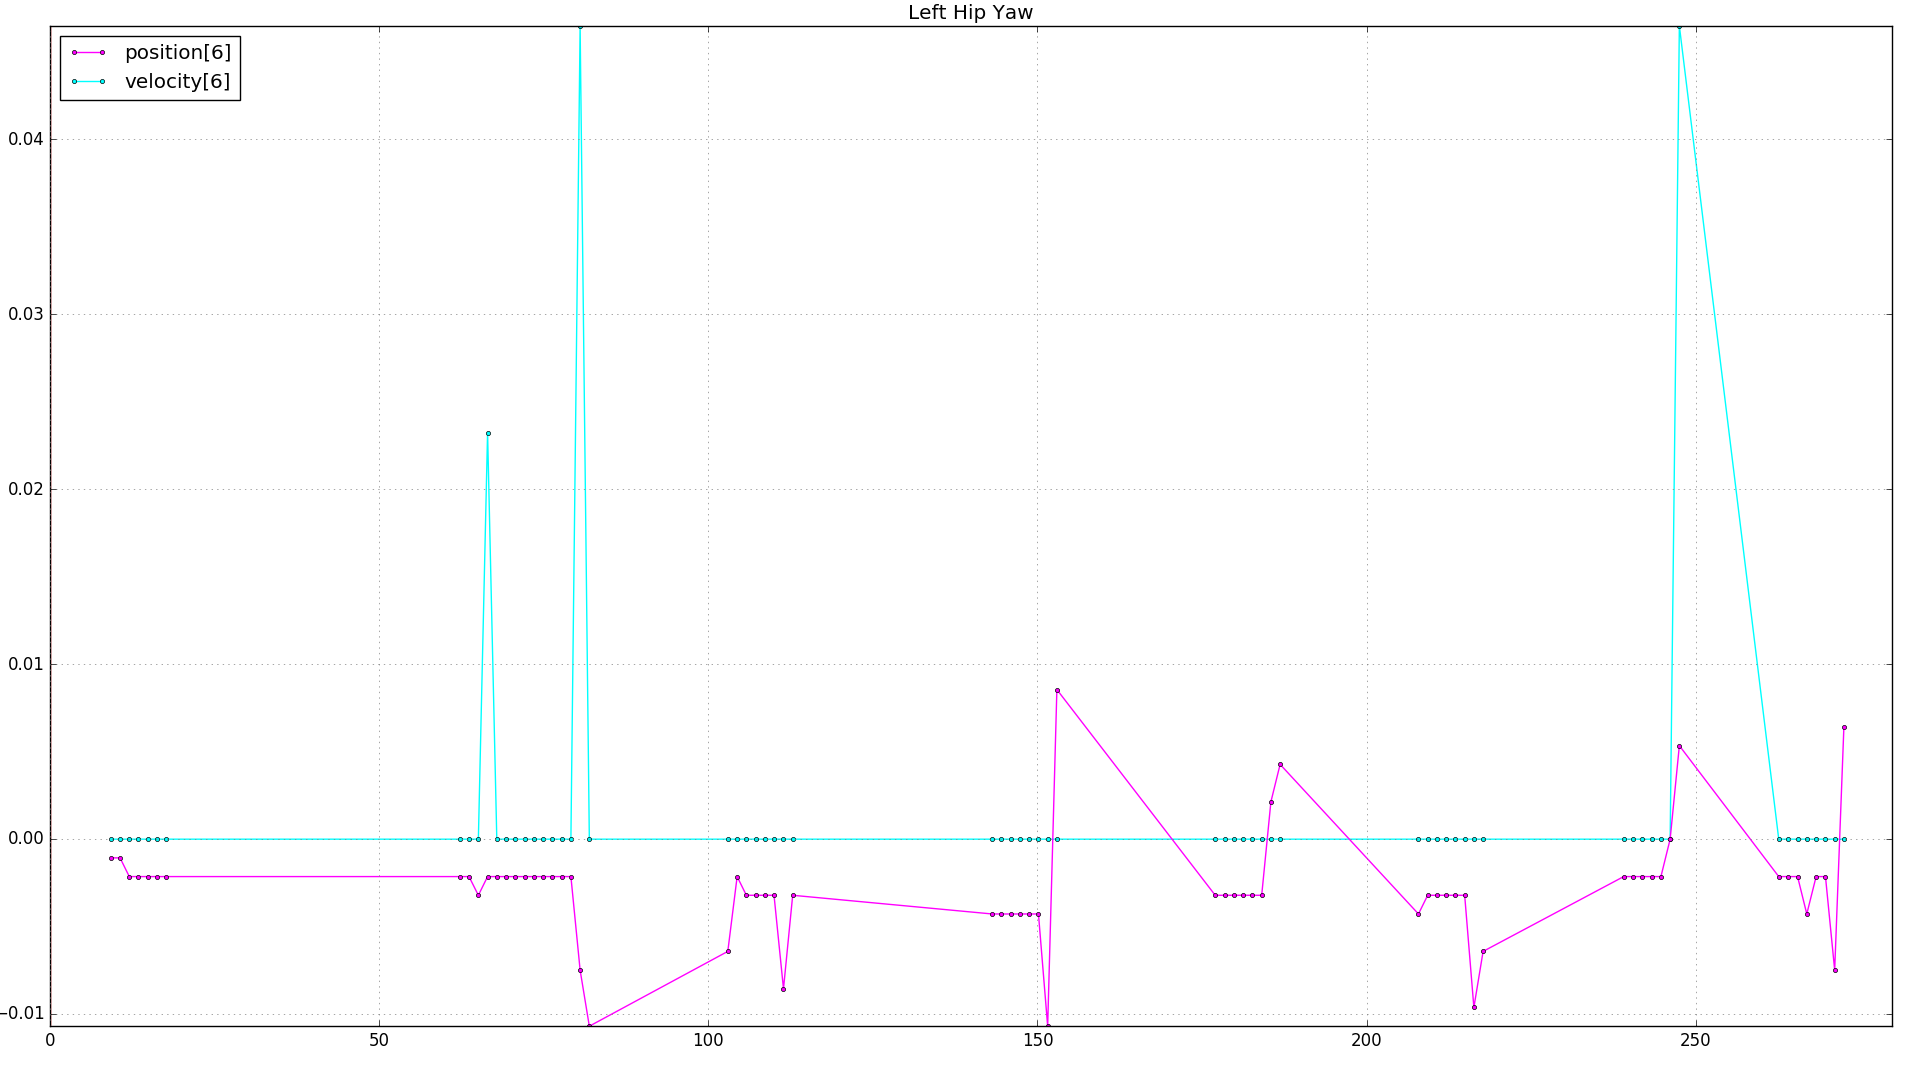
\includegraphics[width=1.0\linewidth]{chapter4/images/left_hip_yaw.png}
  \caption{รูปการสั่งงานข้อต่อ left hip yaw}
  \label{fig:left_hip_yaw}
\end{figure}

\begin{figure}[!ht]
  \centering
  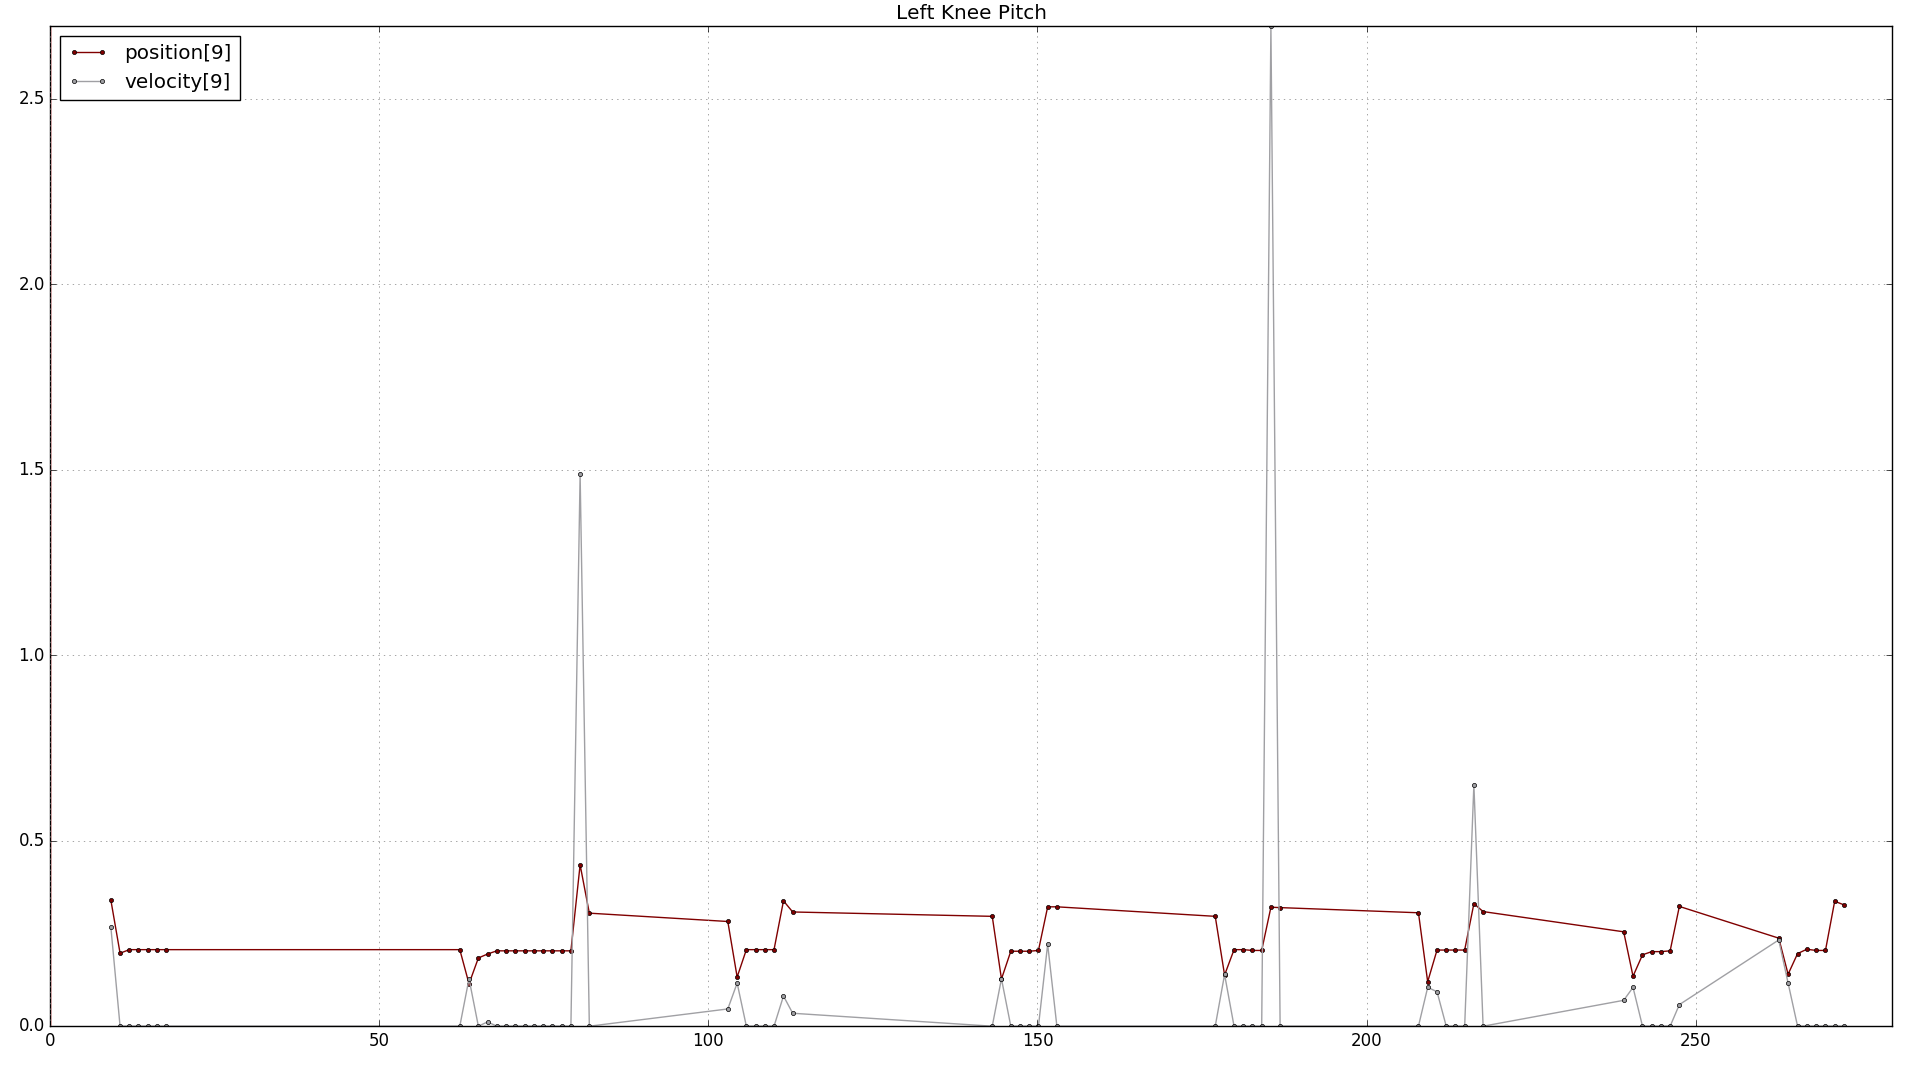
\includegraphics[width=1.0\linewidth]{chapter4/images/left_knee_pitch.png}
  \caption{รูปการสั่งงานข้อต่อ left knee pitch}
  \label{fig:left_knee_pitch}
\end{figure}
\clearpage

\begin{figure}[!ht]
  \centering
  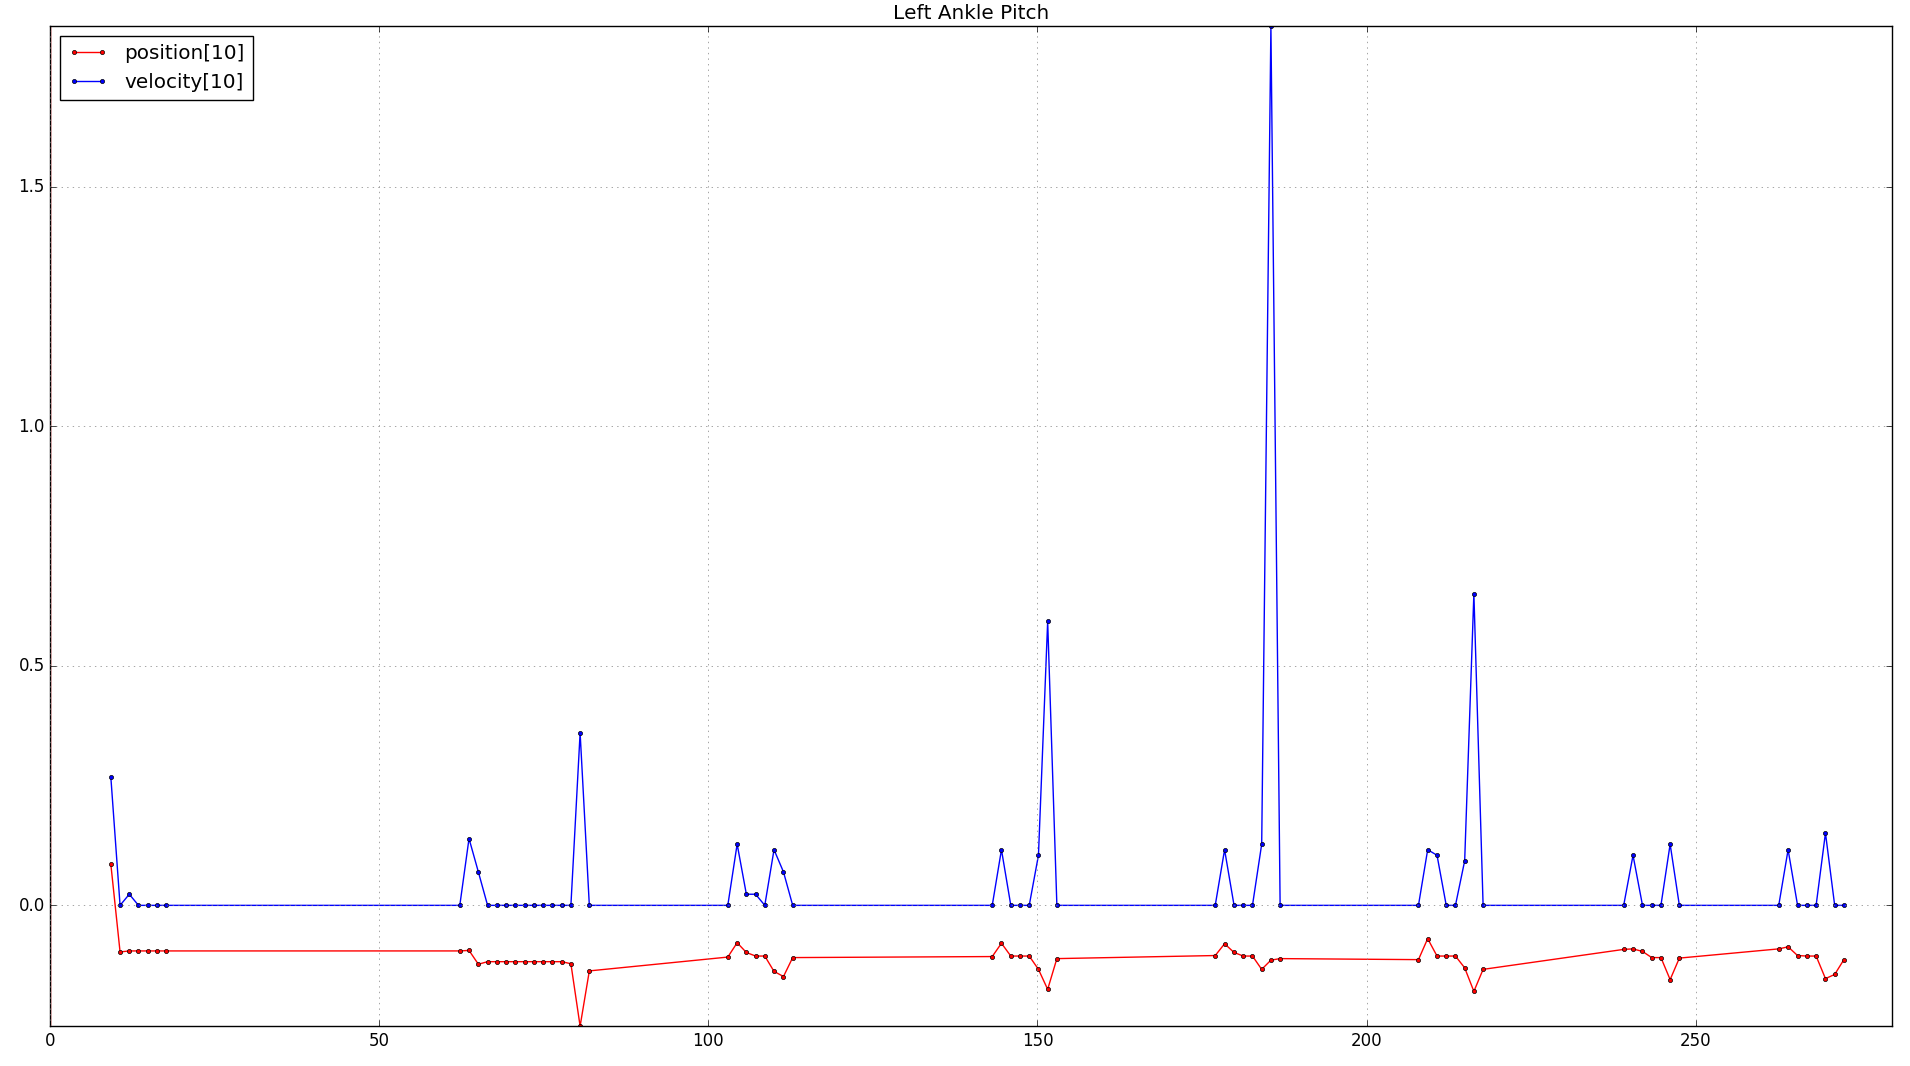
\includegraphics[width=1.0\linewidth]{chapter4/images/left_ankle_pitch.png}
  \caption{รูปการสั่งงานข้อต่อ left ankle pitch}
  \label{fig:left_ankle_pitch}
\end{figure}

\begin{figure}[!ht]
  \centering
  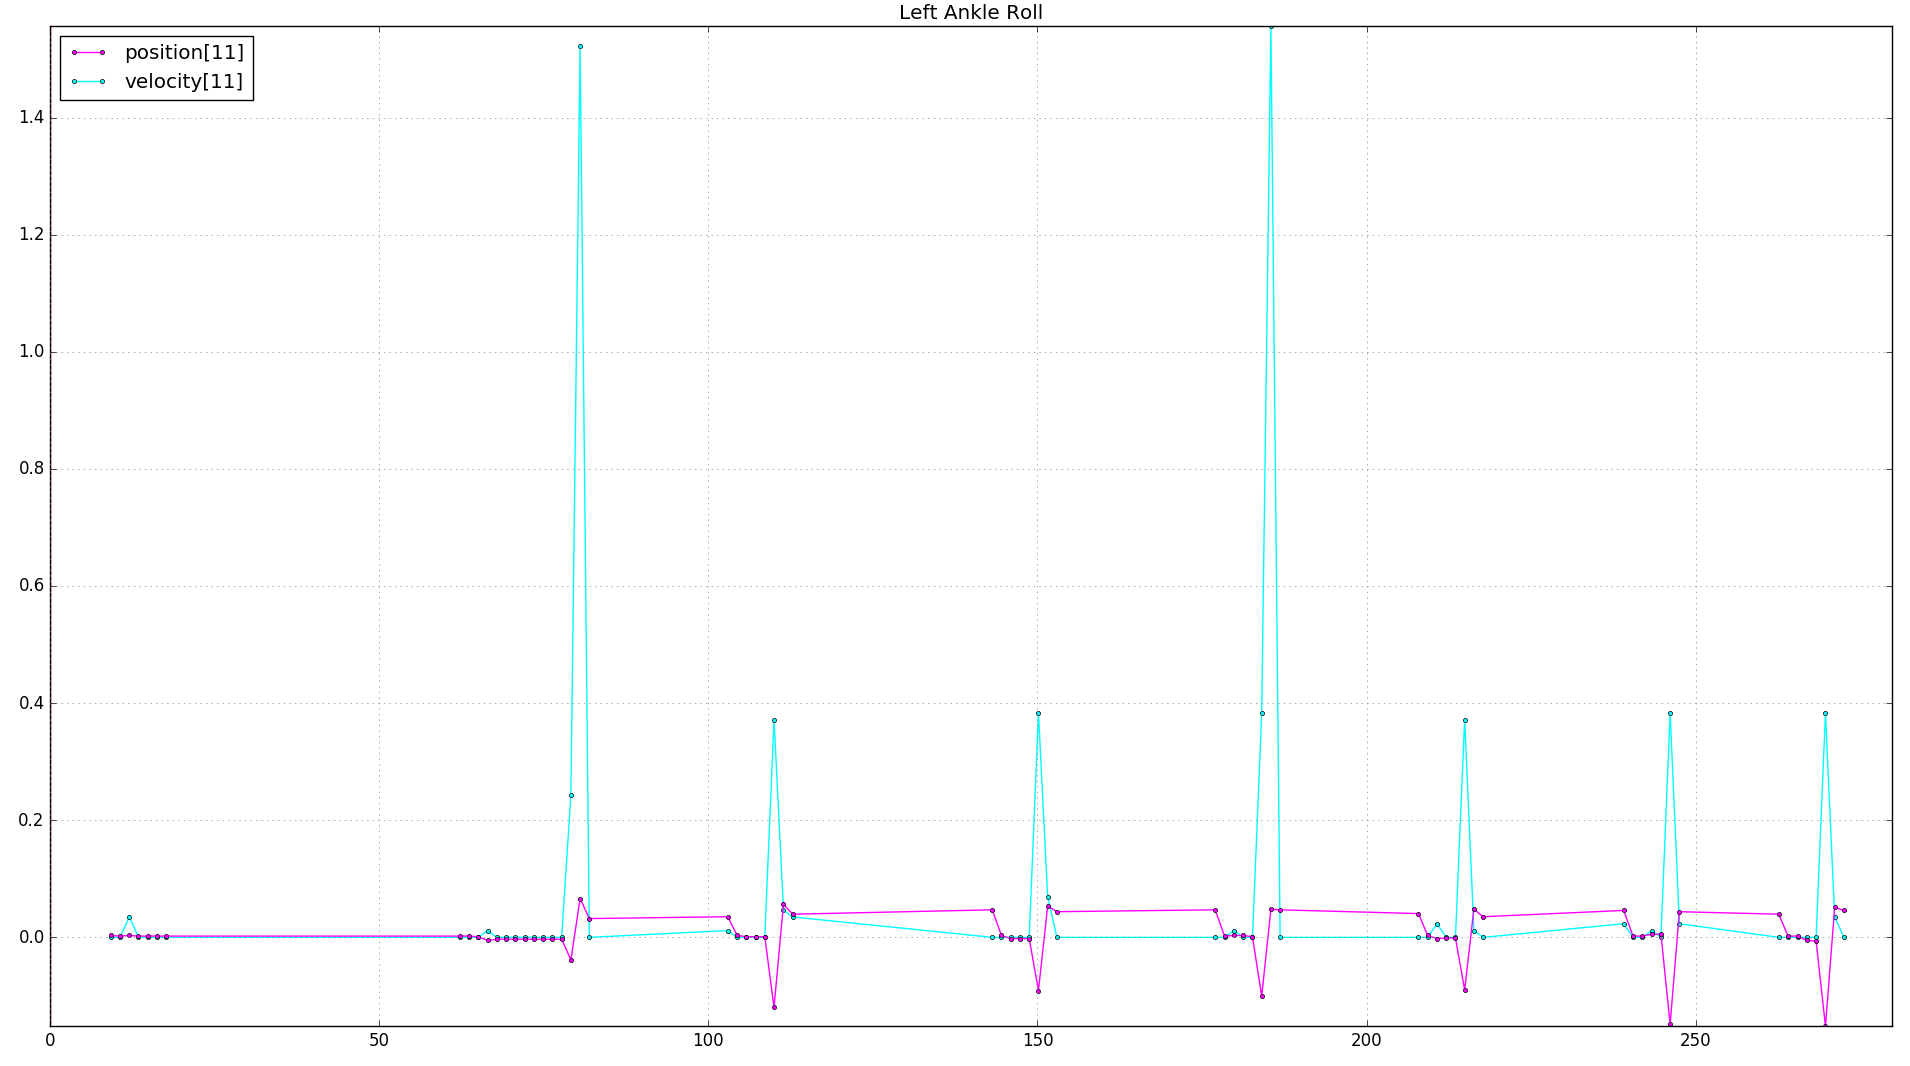
\includegraphics[width=1.0\linewidth]{chapter4/images/left_ankle_roll.png}
  \caption{รูปการสั่งงานข้อต่อ left ankle roll}
  \label{fig:left_ankle_roll}
\end{figure} 
\clearpage

จากกราฟที่แสดงข้างต้นนั้นแสดงถึงตำแหน่งที่สั่งงานให้หุ่นยนต์ขยับในองศาต่างๆของข้อต่อ โดยจะสามารถสังเกตได้จาก
จุด peak ของแต่ละกราฟซึ่งมี 7 จุดในแต่ละกราฟที่เกิดขึ้นในคาบที่ไกล้เคียงกัน โดยค่าในแกน x แสดงถึงช่วงเวลาที่สั่งงานเป็นวินาที 
และแกน y แสดงองศาของมอเตอร์ในหน่วยเรเดียล โดยในการทดลองนี้ เป็นการกำหนดค่าเพื่อทดลองให้หุ่นยนต์มีการเดินเกิดขึ้น
และทดสอบโครงสร้างขณะทำการทดลองอีกด้วย ซึ่งผลการทดลองที่ได้จะพบว่าการเดินครั้งที่ 1-4 เกิดการล้มขึ้น และหลังจากครั้งที่ 5 เป็นต้นไป
หุ่นยนต์สามารถเดินได้ 1 ก้าวจากการทดลองเปลี่ยนค่าให้เหมาะสมกับระบบ ดังแสดงในรูปภาพต่อไปนี้

\begin{figure}[!ht]
    \centering
    \begin{subfigure}[b]{0.4\linewidth}
      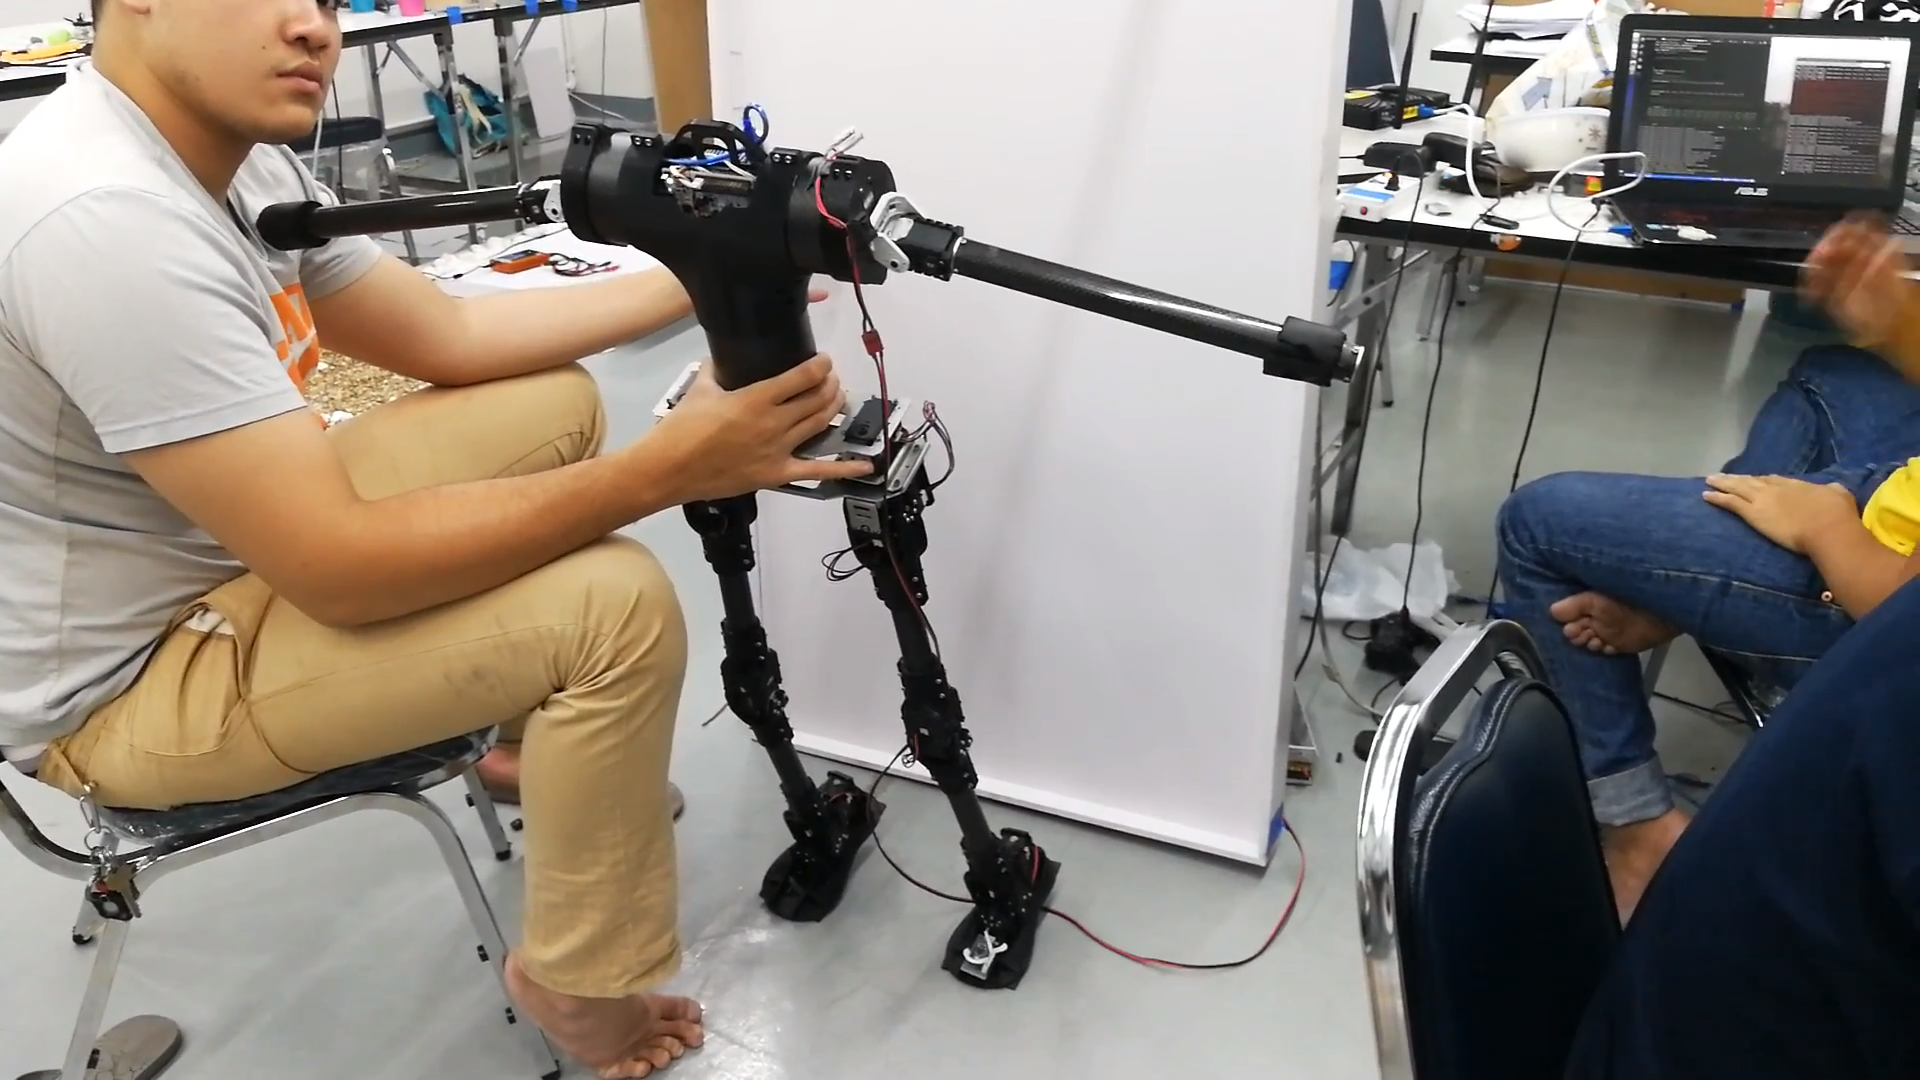
\includegraphics[width=\linewidth]{chapter4/images/fall1.png}
      \caption{รูปการล้มครั้งที่ 1}
    \end{subfigure}
    \begin{subfigure}[b]{0.4\linewidth}
      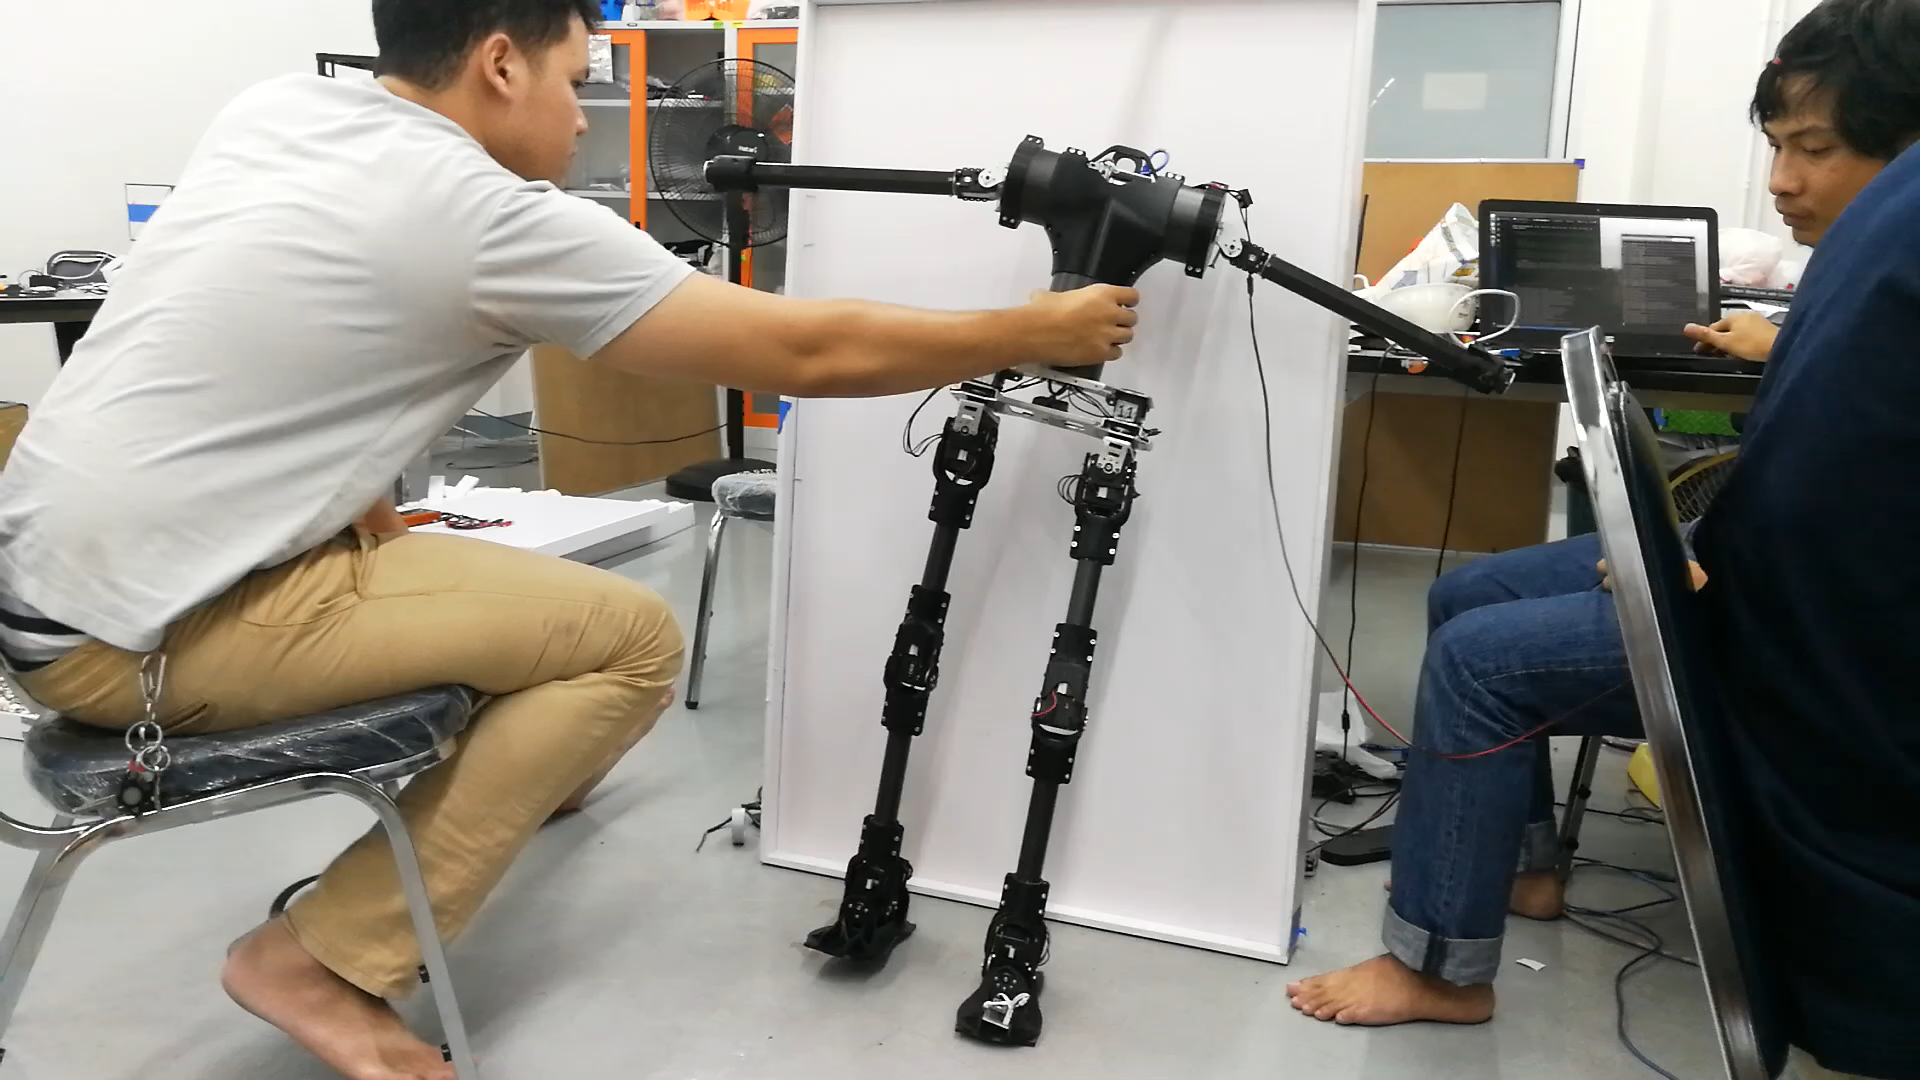
\includegraphics[width=\linewidth]{chapter4/images/fall2.png}
      \caption{รูปการล้มครั้งที่ 2}
    \end{subfigure}
    \begin{subfigure}[b]{0.4\linewidth}
      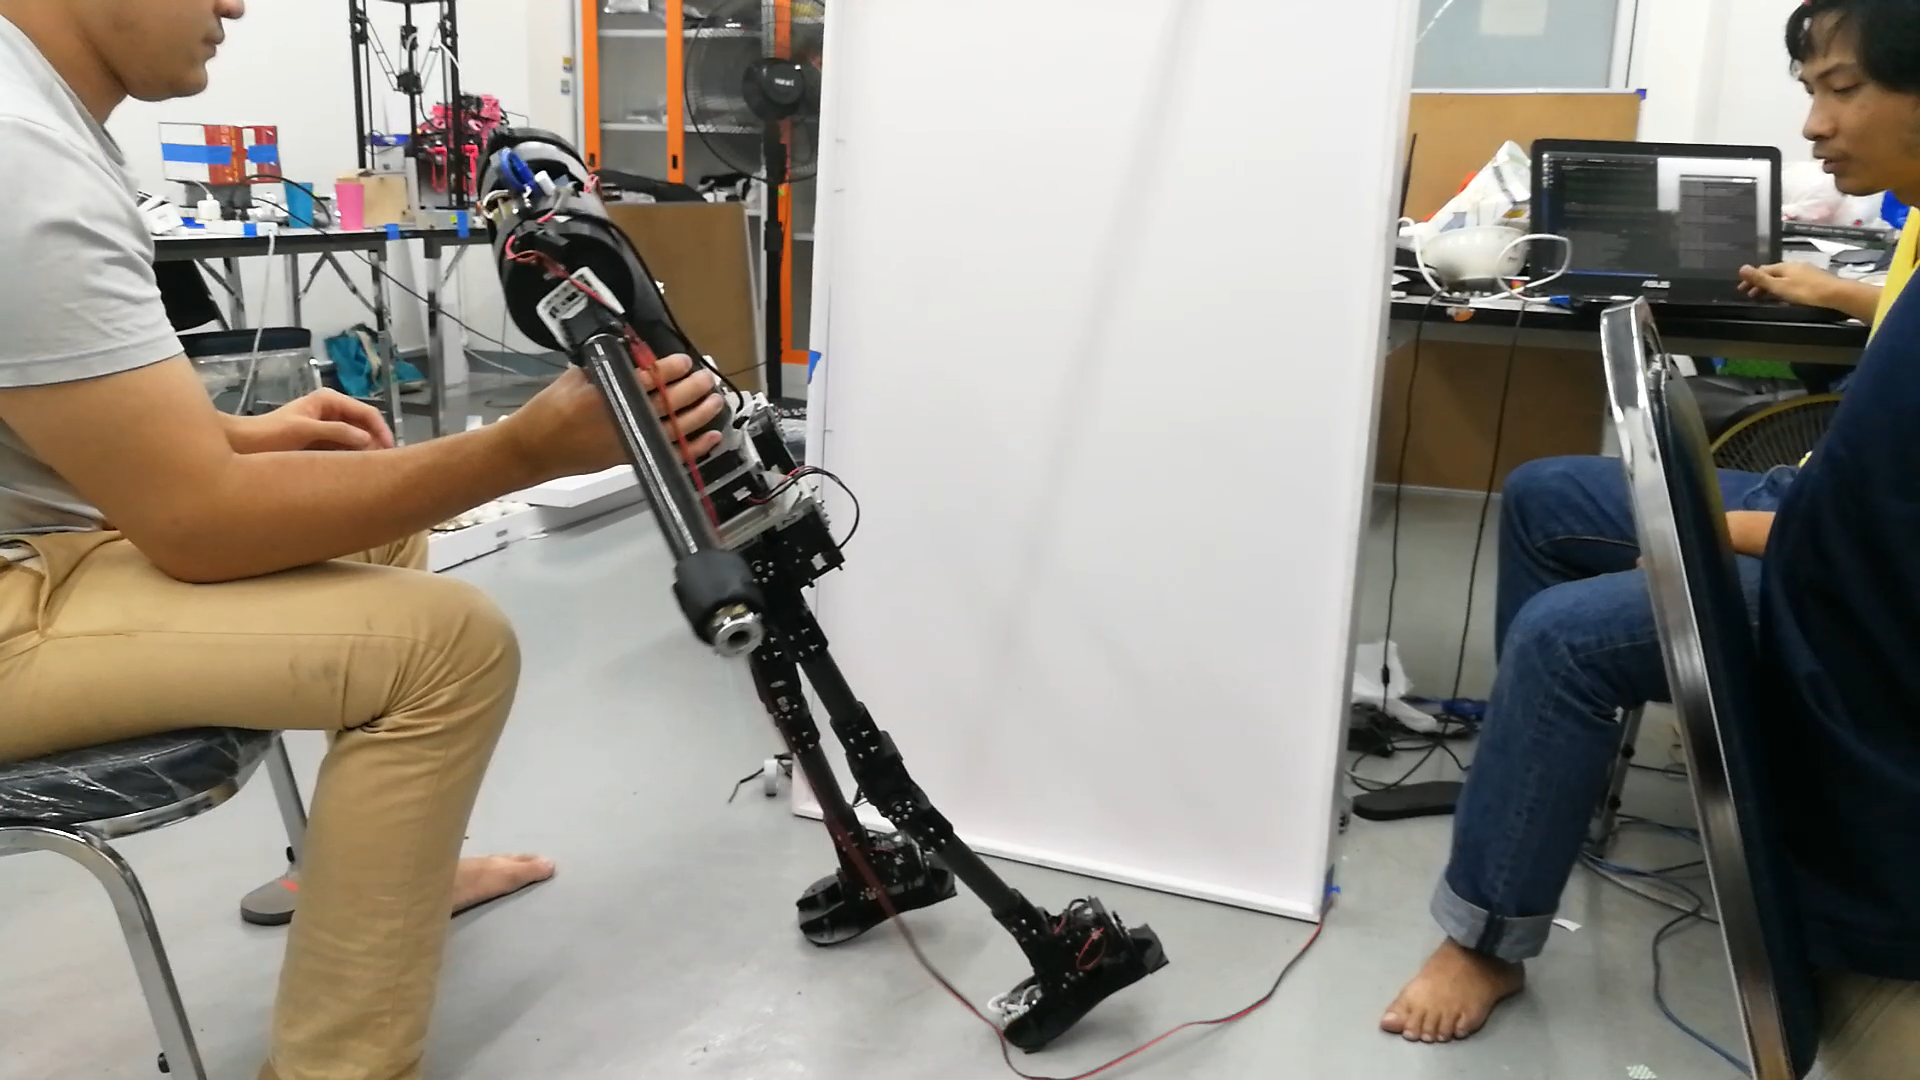
\includegraphics[width=\linewidth]{chapter4/images/fall3.png}
      \caption{รูปการล้มครั้งที่ 3}
    \end{subfigure}
    \begin{subfigure}[b]{0.4\linewidth}
      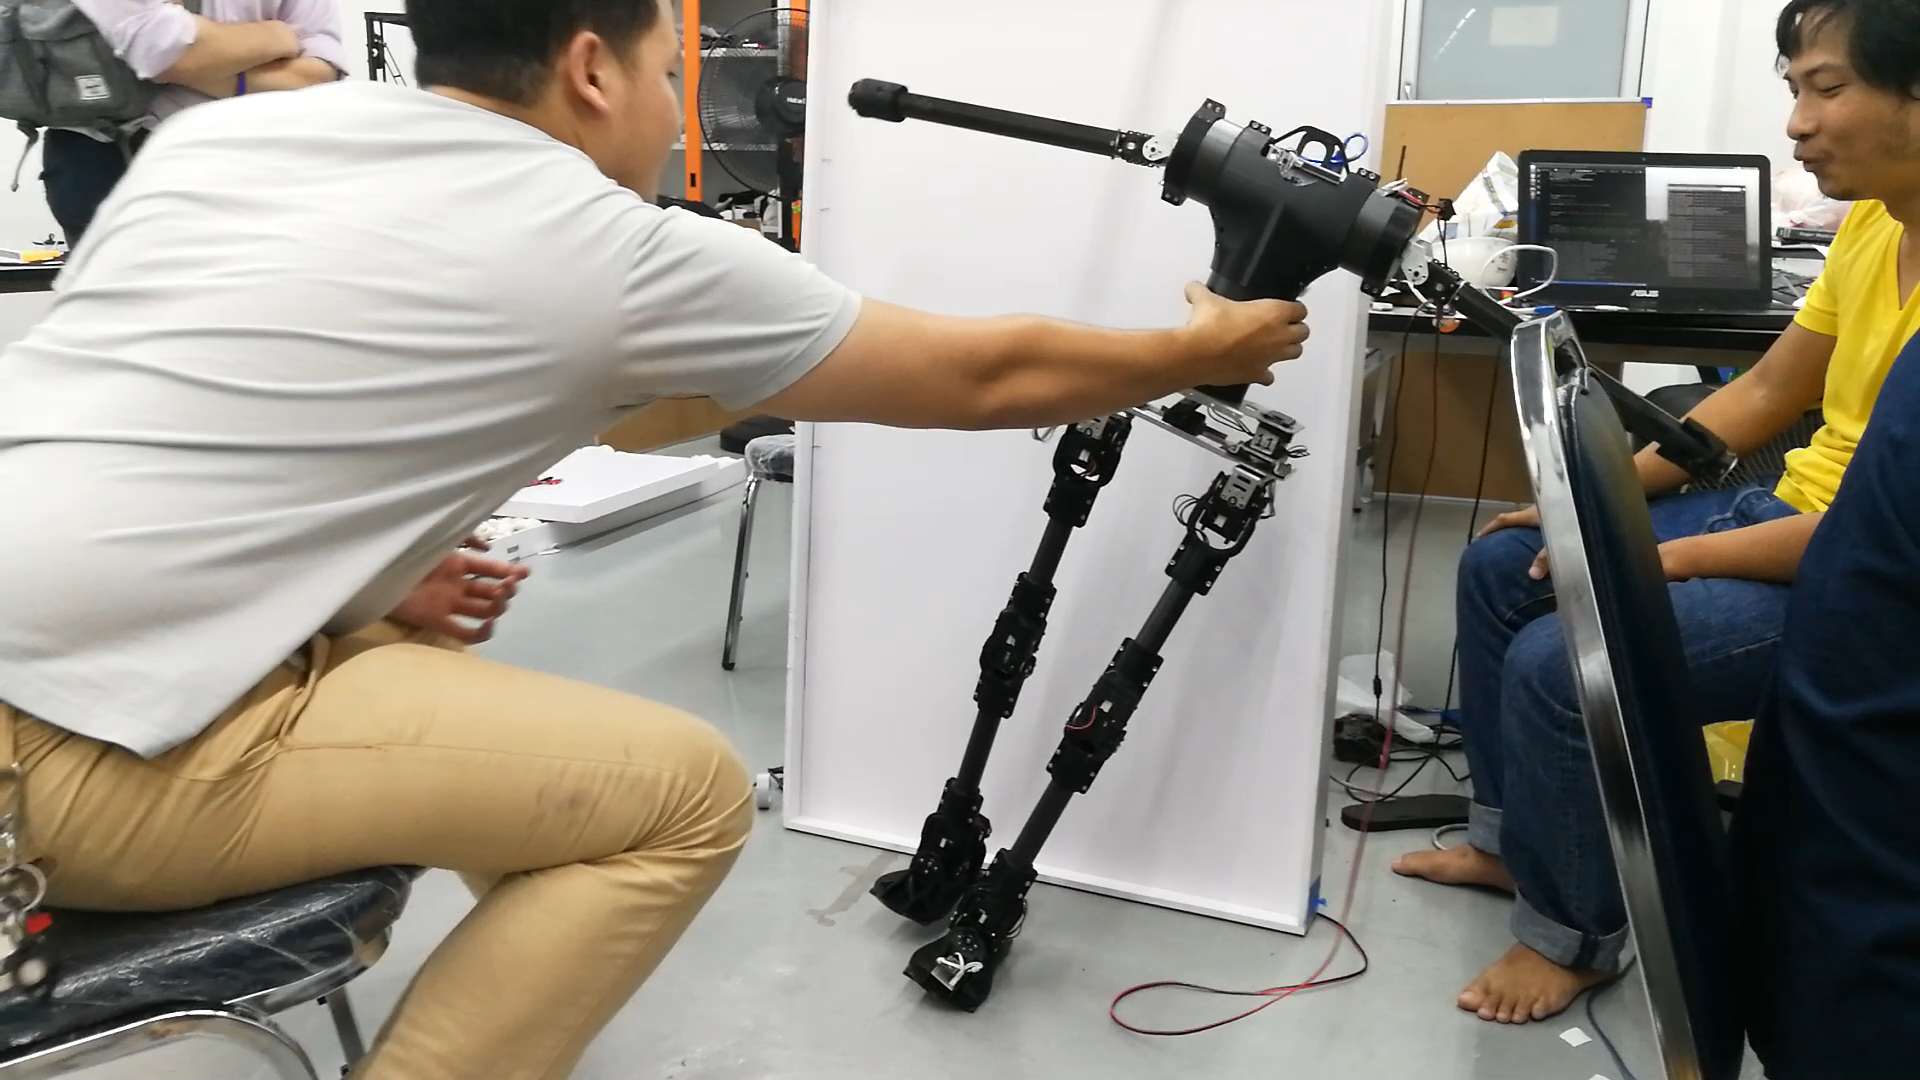
\includegraphics[width=\linewidth]{chapter4/images/fall4.png}
      \caption{รูปการล้มครั้งที่ 4}
    \end{subfigure}
    \begin{subfigure}[b]{0.4\linewidth}
      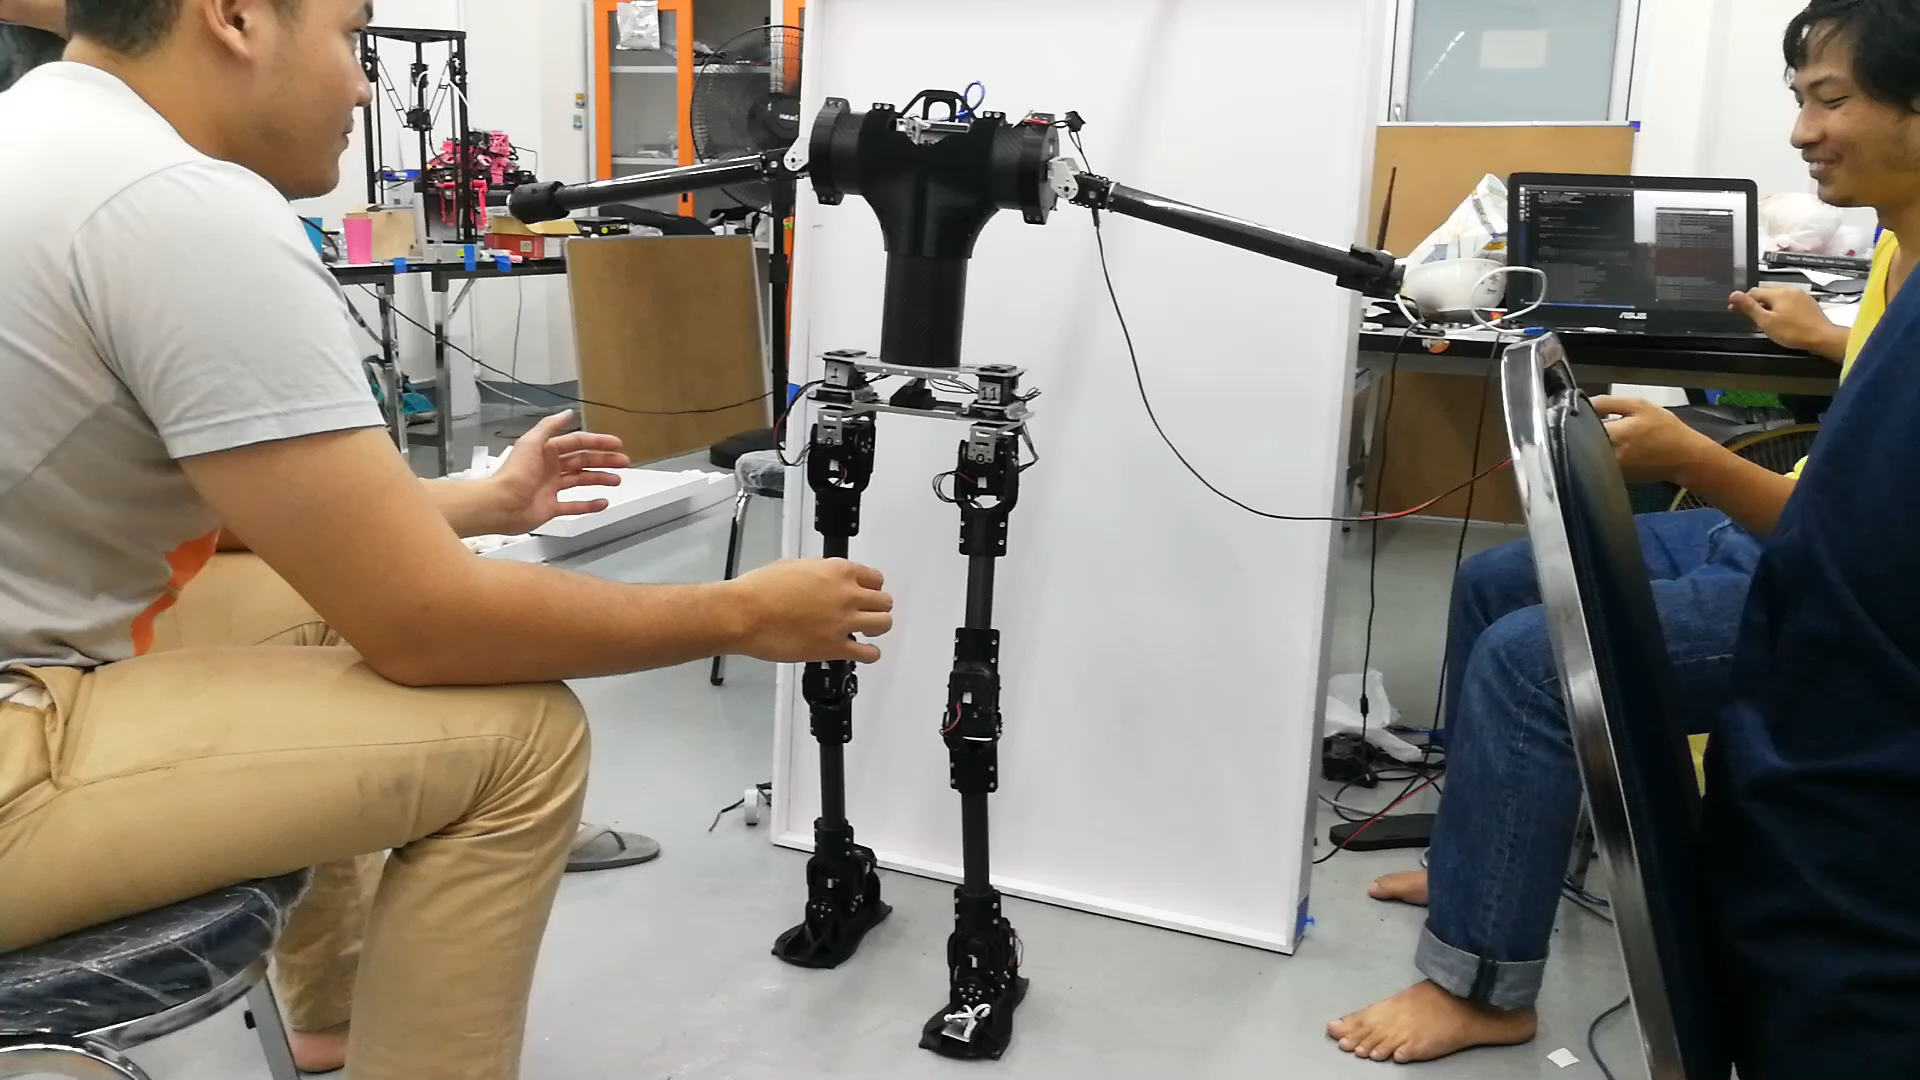
\includegraphics[width=\linewidth]{chapter4/images/achive1.png}
      \caption{รูปการก้าวสำเร็จ}
    \end{subfigure}
    \caption{รูปการทดลองการเดินของหุ่นยนต์ UTHAI}
    \label{fig:test_result}
  \end{figure}


\clearpage
\subsection{ปัญหาที่พบและการแก้ไข}
\subsubsection{อุณหภูมิ}
เมื่อมีการใช้งานเป็นเวลานานจะส่งผลให้มอเตอร์ส่วนสะโพกและข้อเท้ามีความร้อนสูงถึง 50 องศาเซลเซียส 
เนื่องจากมีการสั่งงานให้มอเตอร์อยู่ในตำแหน่งที่กำหนด ซึ่งเมื่อมีแรงบิดข้างนอกมาเกี่ยวข้อง จะทำให้มอเตอร์นั้น
พยายามรักษามุมของตนเองไว้ ส่งผลให้เกิดความร้อนเกิดขึ้นและ ส่งผลให้มอเตอร์อ่อนแรงลงเนื่องจากความร้อนที่เกิดขึ้น 
ในการแก้ไขปัญหานี้สามารถเพิ่มเติมส่วนของการระบายอากาศซึ่งจะส่งผลให้ตัวของหุ่นยนต์นั้นมีน้ำหนักมากขึ้น หรือ หยุดการทดลอง
ไว้สักระยะเพื่อให้มีการระบายอากาศให้อยู่ในอุณหภูมิปกติ
\subsubsection{โครงสร้าง}
เนื่องจากการยึดท่อคาร์บอนไฟเบอร์นั้นได้ทำการยึดด้วยการบีบอัดเพื่อให้เกิดแรงเสียดทางสูงแต่ว่าเมื่อมีการ สั่งงานที่มีการกระชากกล่าวคือ
มีการเคลื่อนที่ของมุมมอเตอร์ที่มีความแร็วสูง จะส่งผลให้เกิดแรงบิดตามแนวแกนซึ่งเกินแรงเสียดทานที่การยึดติดจะรับไหว จึงเกิดการบิด ของข้อต่อ
เกิดขึ้น ส่งผลให้ ส่วนของเท้ามีการบิดไปจากท่าปกติ ซึ่งสามารถแก้ไขได้โดยเพิ่มแรงยึดด้วยการเสริมแผ่นยางบางๆบริเวณหน้าสัมผัสที่ติดกับท่อคาร์บอนไฟเบอร์
เพื่อเพิ่มแรงยึดไปอีกขั้นหนึ่ง 
\subsubsection{มอเตอร์}
เนื่องจากว่าตัวหุ่นยนต์มีการใช้มอเตอร์ในการขับเคลื่อนโดยตรงกับข้อต่อ ซึ่งเป็นผลทำให้ต้องใช้มอเตอร์ที่มีแรงบิดสูง
เพื่อขับเคลื่อนให้โครงสร้างมีการขยับตัวได้ แต่เนื่องจากว่าตัวหุ่นยนต์นั้นออกแบบมาให้มีความสูงที่ระดับ 1 เมตร ซึ่งหมายถึงจะมีแรง
โมเมนต์ที่เกิดขึ้นกับข้อต่อเมื่อหุ่นยนต์มีการก้าวเท้าหรือขยับตัว เป็นผลทำให้เกิด backlash เนื่องจากว่าตัวของมอเตอร์เองไม่สามารถควบคุมตำแหน่งของตนเองให้อยู่
ในมุมที่สั้งงานไว้ได้ จึงแก้ไขปัญหาโดยการเพิ่มระยะการสั่งงานเพื่อให้ครอบคลุมช่วง blacklash เพื่อที่จะให้ไปยังมุมที่ต้องการได้ และยังเพิ่มกำลังไฟให้กับมอเตอร์
จาก 12V เป็น 14V เพื่อให้มีแรงบิดที่เพิ่มมากขึ้นกว่าเดิม ซึ่งจะส่งให้ backlash น้อยลงและสามารถคุมตำแหน่งงายขึ้น


